\documentclass[a4paper,11pt]{article}

\usepackage{polski}
\usepackage[utf8]{inputenc}
\usepackage{graphicx}
\usepackage{xcolor}
\usepackage[fleqn]{amsmath}
\usepackage{tgtermes}

\usepackage[
pdftitle={Bazy danych},
pdfauthor={evemorgen, AGH},
colorlinks=true,linkcolor=blue,urlcolor=blue,citecolor=blue,bookmarks=true,
bookmarksopenlevel=2]{hyperref}
\usepackage{amsmath,amssymb,amsthm,textcomp}
\usepackage{enumerate}
\usepackage{multicol}
\usepackage{tikz}
\usepackage{geometry}
\geometry{
 a4paper,
 total={170mm,257mm},
 left=20mm,
 top=20mm,
}


% custom footers and headers
\usepackage{fancyhdr,lastpage}
\pagestyle{fancy}
\lhead{}
\chead{}
\rhead{}
\lfoot{Assignment \textnumero{} 1}
\cfoot{}
\rfoot{Page \thepage\ /\ \pageref*{LastPage}}
\renewcommand{\headrulewidth}{0pt}
\renewcommand{\footrulewidth}{0pt}
%

%%%----------%%%----------%%%----------%%%----------%%%

\begin{document}

\title{Bazy danych - 1}
\author{evemorgen, AGH}
\date{22/11/2016}
\maketitle

\section{Narysuj diagram związków encji według poniższego opisu.}
\begin{itemize}
	\item Każda firma ma 4 działy, a każdy dział należy do jednej firmy.
	\item Każdy dział ma przynajmniej jednego pracownika, a każdy pracownik pracuje w jednym dziale.
	\item Każdy pracownik może mieć (lub nie mieć) przynajmniej jednego podwładnego, a każdy podwładny ma jednego zwierzchnika.
	\item Każdy pracownik może mieć (lub nie mieć) historię swojego zatrudnienia.
\end{itemize}

% Graphic for TeX using PGF
% Title: /Users/evemorgen/Dropbox/studia/3rokEaiib/bazy_danych/lab7/7-1.dia
% Creator: Dia v0.97.2
% CreationDate: Mon Nov 21 23:59:25 2016
% For: evemorgen
% \usepackage{tikz}
% The following commands are not supported in PSTricks at present
% We define them conditionally, so when they are implemented,
% this pgf file will use them.
\ifx\du\undefined
  \newlength{\du}
\fi
\setlength{\du}{15\unitlength}
\begin{tikzpicture}
\pgftransformxscale{1.000000}
\pgftransformyscale{-1.000000}
\definecolor{dialinecolor}{rgb}{0.000000, 0.000000, 0.000000}
\pgfsetstrokecolor{dialinecolor}
\definecolor{dialinecolor}{rgb}{1.000000, 1.000000, 1.000000}
\pgfsetfillcolor{dialinecolor}
\pgfsetlinewidth{0.100000\du}
\pgfsetdash{}{0pt}
\definecolor{dialinecolor}{rgb}{1.000000, 1.000000, 1.000000}
\pgfsetfillcolor{dialinecolor}
\fill (1.450000\du,10.650000\du)--(1.450000\du,12.050000\du)--(5.030000\du,12.050000\du)--(5.030000\du,10.650000\du)--cycle;
\definecolor{dialinecolor}{rgb}{0.000000, 0.000000, 0.000000}
\pgfsetstrokecolor{dialinecolor}
\draw (1.450000\du,10.650000\du)--(1.450000\du,12.050000\du)--(5.030000\du,12.050000\du)--(5.030000\du,10.650000\du)--cycle;
% setfont left to latex
\definecolor{dialinecolor}{rgb}{0.000000, 0.000000, 0.000000}
\pgfsetstrokecolor{dialinecolor}
\node at (3.240000\du,11.650000\du){Firmy};
\definecolor{dialinecolor}{rgb}{1.000000, 1.000000, 1.000000}
\pgfsetfillcolor{dialinecolor}
\fill (1.450000\du,12.050000\du)--(1.450000\du,13.050000\du)--(5.030000\du,13.050000\du)--(5.030000\du,12.050000\du)--cycle;
\definecolor{dialinecolor}{rgb}{0.000000, 0.000000, 0.000000}
\pgfsetstrokecolor{dialinecolor}
\draw (1.450000\du,12.050000\du)--(1.450000\du,13.050000\du)--(5.030000\du,13.050000\du)--(5.030000\du,12.050000\du)--cycle;
% setfont left to latex
\definecolor{dialinecolor}{rgb}{0.000000, 0.000000, 0.000000}
\pgfsetstrokecolor{dialinecolor}
\node[anchor=west] at (1.600000\du,12.750000\du){\#firmaID};
\definecolor{dialinecolor}{rgb}{1.000000, 1.000000, 1.000000}
\pgfsetfillcolor{dialinecolor}
\fill (1.450000\du,13.050000\du)--(1.450000\du,13.450000\du)--(5.030000\du,13.450000\du)--(5.030000\du,13.050000\du)--cycle;
\definecolor{dialinecolor}{rgb}{0.000000, 0.000000, 0.000000}
\pgfsetstrokecolor{dialinecolor}
\draw (1.450000\du,13.050000\du)--(1.450000\du,13.450000\du)--(5.030000\du,13.450000\du)--(5.030000\du,13.050000\du)--cycle;
\pgfsetlinewidth{0.100000\du}
\pgfsetdash{}{0pt}
\definecolor{dialinecolor}{rgb}{1.000000, 1.000000, 1.000000}
\pgfsetfillcolor{dialinecolor}
\fill (11.265000\du,10.640000\du)--(11.265000\du,12.040000\du)--(14.845000\du,12.040000\du)--(14.845000\du,10.640000\du)--cycle;
\definecolor{dialinecolor}{rgb}{0.000000, 0.000000, 0.000000}
\pgfsetstrokecolor{dialinecolor}
\draw (11.265000\du,10.640000\du)--(11.265000\du,12.040000\du)--(14.845000\du,12.040000\du)--(14.845000\du,10.640000\du)--cycle;
% setfont left to latex
\definecolor{dialinecolor}{rgb}{0.000000, 0.000000, 0.000000}
\pgfsetstrokecolor{dialinecolor}
\node at (13.055000\du,11.640000\du){Działy};
\definecolor{dialinecolor}{rgb}{1.000000, 1.000000, 1.000000}
\pgfsetfillcolor{dialinecolor}
\fill (11.265000\du,12.040000\du)--(11.265000\du,13.040000\du)--(14.845000\du,13.040000\du)--(14.845000\du,12.040000\du)--cycle;
\definecolor{dialinecolor}{rgb}{0.000000, 0.000000, 0.000000}
\pgfsetstrokecolor{dialinecolor}
\draw (11.265000\du,12.040000\du)--(11.265000\du,13.040000\du)--(14.845000\du,13.040000\du)--(14.845000\du,12.040000\du)--cycle;
% setfont left to latex
\definecolor{dialinecolor}{rgb}{0.000000, 0.000000, 0.000000}
\pgfsetstrokecolor{dialinecolor}
\node[anchor=west] at (11.415000\du,12.740000\du){\#działID};
\definecolor{dialinecolor}{rgb}{1.000000, 1.000000, 1.000000}
\pgfsetfillcolor{dialinecolor}
\fill (11.265000\du,13.040000\du)--(11.265000\du,13.440000\du)--(14.845000\du,13.440000\du)--(14.845000\du,13.040000\du)--cycle;
\definecolor{dialinecolor}{rgb}{0.000000, 0.000000, 0.000000}
\pgfsetstrokecolor{dialinecolor}
\draw (11.265000\du,13.040000\du)--(11.265000\du,13.440000\du)--(14.845000\du,13.440000\du)--(14.845000\du,13.040000\du)--cycle;
\pgfsetlinewidth{0.100000\du}
\pgfsetdash{}{0pt}
\definecolor{dialinecolor}{rgb}{1.000000, 1.000000, 1.000000}
\pgfsetfillcolor{dialinecolor}
\fill (19.580000\du,10.630000\du)--(19.580000\du,12.030000\du)--(25.235000\du,12.030000\du)--(25.235000\du,10.630000\du)--cycle;
\definecolor{dialinecolor}{rgb}{0.000000, 0.000000, 0.000000}
\pgfsetstrokecolor{dialinecolor}
\draw (19.580000\du,10.630000\du)--(19.580000\du,12.030000\du)--(25.235000\du,12.030000\du)--(25.235000\du,10.630000\du)--cycle;
% setfont left to latex
\definecolor{dialinecolor}{rgb}{0.000000, 0.000000, 0.000000}
\pgfsetstrokecolor{dialinecolor}
\node at (22.407500\du,11.630000\du){Pracownicy};
\definecolor{dialinecolor}{rgb}{1.000000, 1.000000, 1.000000}
\pgfsetfillcolor{dialinecolor}
\fill (19.580000\du,12.030000\du)--(19.580000\du,13.030000\du)--(25.235000\du,13.030000\du)--(25.235000\du,12.030000\du)--cycle;
\definecolor{dialinecolor}{rgb}{0.000000, 0.000000, 0.000000}
\pgfsetstrokecolor{dialinecolor}
\draw (19.580000\du,12.030000\du)--(19.580000\du,13.030000\du)--(25.235000\du,13.030000\du)--(25.235000\du,12.030000\du)--cycle;
% setfont left to latex
\definecolor{dialinecolor}{rgb}{0.000000, 0.000000, 0.000000}
\pgfsetstrokecolor{dialinecolor}
\node[anchor=west] at (19.730000\du,12.730000\du){\#pracownikID};
\definecolor{dialinecolor}{rgb}{1.000000, 1.000000, 1.000000}
\pgfsetfillcolor{dialinecolor}
\fill (19.580000\du,13.030000\du)--(19.580000\du,13.430000\du)--(25.235000\du,13.430000\du)--(25.235000\du,13.030000\du)--cycle;
\definecolor{dialinecolor}{rgb}{0.000000, 0.000000, 0.000000}
\pgfsetstrokecolor{dialinecolor}
\draw (19.580000\du,13.030000\du)--(19.580000\du,13.430000\du)--(25.235000\du,13.430000\du)--(25.235000\du,13.030000\du)--cycle;
\pgfsetlinewidth{0.100000\du}
\pgfsetdash{}{0pt}
\definecolor{dialinecolor}{rgb}{1.000000, 1.000000, 1.000000}
\pgfsetfillcolor{dialinecolor}
\fill (31.995000\du,10.920000\du)--(31.995000\du,12.320000\du)--(36.032500\du,12.320000\du)--(36.032500\du,10.920000\du)--cycle;
\definecolor{dialinecolor}{rgb}{0.000000, 0.000000, 0.000000}
\pgfsetstrokecolor{dialinecolor}
\draw (31.995000\du,10.920000\du)--(31.995000\du,12.320000\du)--(36.032500\du,12.320000\du)--(36.032500\du,10.920000\du)--cycle;
% setfont left to latex
\definecolor{dialinecolor}{rgb}{0.000000, 0.000000, 0.000000}
\pgfsetstrokecolor{dialinecolor}
\node at (34.013750\du,11.920000\du){Historia};
\definecolor{dialinecolor}{rgb}{1.000000, 1.000000, 1.000000}
\pgfsetfillcolor{dialinecolor}
\fill (31.995000\du,12.320000\du)--(31.995000\du,12.720000\du)--(36.032500\du,12.720000\du)--(36.032500\du,12.320000\du)--cycle;
\definecolor{dialinecolor}{rgb}{0.000000, 0.000000, 0.000000}
\pgfsetstrokecolor{dialinecolor}
\draw (31.995000\du,12.320000\du)--(31.995000\du,12.720000\du)--(36.032500\du,12.720000\du)--(36.032500\du,12.320000\du)--cycle;
\definecolor{dialinecolor}{rgb}{1.000000, 1.000000, 1.000000}
\pgfsetfillcolor{dialinecolor}
\fill (31.995000\du,12.720000\du)--(31.995000\du,13.120000\du)--(36.032500\du,13.120000\du)--(36.032500\du,12.720000\du)--cycle;
\definecolor{dialinecolor}{rgb}{0.000000, 0.000000, 0.000000}
\pgfsetstrokecolor{dialinecolor}
\draw (31.995000\du,12.720000\du)--(31.995000\du,13.120000\du)--(36.032500\du,13.120000\du)--(36.032500\du,12.720000\du)--cycle;
\pgfsetlinewidth{0.100000\du}
\pgfsetdash{}{0pt}
\pgfsetmiterjoin
\pgfsetbuttcap
{
\definecolor{dialinecolor}{rgb}{0.000000, 0.000000, 0.000000}
\pgfsetfillcolor{dialinecolor}
% was here!!!
\definecolor{dialinecolor}{rgb}{0.000000, 0.000000, 0.000000}
\pgfsetstrokecolor{dialinecolor}
\draw (5.080449\du,12.050000\du)--(8.147500\du,12.050000\du)--(8.147500\du,12.040000\du)--(11.214551\du,12.040000\du);
}
% setfont left to latex
\definecolor{dialinecolor}{rgb}{0.000000, 0.000000, 0.000000}
\pgfsetfillcolor{dialinecolor}
\fill (8.347500\du,12.045000\du)--(8.347500\du,11.645000\du)--(8.747500\du,11.845000\du)--cycle;
\pgfsetlinewidth{0.100000\du}
\pgfsetdash{}{0pt}
\pgfsetmiterjoin
\pgfsetbuttcap
{
\definecolor{dialinecolor}{rgb}{0.000000, 0.000000, 0.000000}
\pgfsetfillcolor{dialinecolor}
% was here!!!
\definecolor{dialinecolor}{rgb}{0.000000, 0.000000, 0.000000}
\pgfsetstrokecolor{dialinecolor}
\draw (14.895449\du,12.040000\du)--(17.212549\du,12.040000\du)--(17.212549\du,12.030000\du)--(19.529649\du,12.030000\du);
}
% setfont left to latex
\definecolor{dialinecolor}{rgb}{0.000000, 0.000000, 0.000000}
\pgfsetfillcolor{dialinecolor}
\fill (17.412549\du,12.035000\du)--(17.412549\du,11.635000\du)--(17.812549\du,11.835000\du)--cycle;
\pgfsetlinewidth{0.100000\du}
\pgfsetdash{}{0pt}
\pgfsetmiterjoin
\pgfsetbuttcap
{
\definecolor{dialinecolor}{rgb}{0.000000, 0.000000, 0.000000}
\pgfsetfillcolor{dialinecolor}
% was here!!!
\definecolor{dialinecolor}{rgb}{0.000000, 0.000000, 0.000000}
\pgfsetstrokecolor{dialinecolor}
\draw (22.407500\du,10.579646\du)--(22.407500\du,9.529646\du)--(34.013750\du,9.529646\du)--(34.013750\du,10.920000\du);
}
% setfont left to latex
\definecolor{dialinecolor}{rgb}{0.000000, 0.000000, 0.000000}
\pgfsetfillcolor{dialinecolor}
\fill (28.310625\du,9.529646\du)--(28.310625\du,9.129646\du)--(28.710625\du,9.329646\du)--cycle;
\pgfsetlinewidth{0.100000\du}
\pgfsetdash{}{0pt}
\pgfsetmiterjoin
\pgfsetbuttcap
{
\definecolor{dialinecolor}{rgb}{0.000000, 0.000000, 0.000000}
\pgfsetfillcolor{dialinecolor}
% was here!!!
\definecolor{dialinecolor}{rgb}{0.000000, 0.000000, 0.000000}
\pgfsetstrokecolor{dialinecolor}
\draw (25.235000\du,11.330000\du)--(27.950000\du,11.330000\du)--(27.950000\du,13.250000\du)--(25.300000\du,13.250000\du);
}
% setfont left to latex
\definecolor{dialinecolor}{rgb}{0.000000, 0.000000, 0.000000}
\pgfsetfillcolor{dialinecolor}
\fill (28.150000\du,12.290000\du)--(28.150000\du,11.890000\du)--(28.550000\du,12.090000\du)--cycle;
% setfont left to latex
\definecolor{dialinecolor}{rgb}{0.000000, 0.000000, 0.000000}
\pgfsetstrokecolor{dialinecolor}
\node at (8.200000\du,11.265000\du){Posiadają};
% setfont left to latex
\definecolor{dialinecolor}{rgb}{0.000000, 0.000000, 0.000000}
\pgfsetstrokecolor{dialinecolor}
\node at (17.200000\du,11.315000\du){ma};
% setfont left to latex
\definecolor{dialinecolor}{rgb}{0.000000, 0.000000, 0.000000}
\pgfsetstrokecolor{dialinecolor}
\node at (27.500000\du,11.076125\du){pracownik};
% setfont left to latex
\definecolor{dialinecolor}{rgb}{0.000000, 0.000000, 0.000000}
\pgfsetstrokecolor{dialinecolor}
\node at (27.350000\du,14.076125\du){podwładny};
% setfont left to latex
\definecolor{dialinecolor}{rgb}{0.000000, 0.000000, 0.000000}
\pgfsetstrokecolor{dialinecolor}
\node at (28.400000\du,8.626125\du){mają};
% setfont left to latex
\definecolor{dialinecolor}{rgb}{0.000000, 0.000000, 0.000000}
\pgfsetstrokecolor{dialinecolor}
\node at (35.050000\du,10.426125\du){0..1};
% setfont left to latex
\definecolor{dialinecolor}{rgb}{0.000000, 0.000000, 0.000000}
\pgfsetstrokecolor{dialinecolor}
\node at (21.050000\du,10.176125\du){1..1};
% setfont left to latex
\definecolor{dialinecolor}{rgb}{0.000000, 0.000000, 0.000000}
\pgfsetstrokecolor{dialinecolor}
\node at (26.000000\du,11.926125\du){1..1};
% setfont left to latex
\definecolor{dialinecolor}{rgb}{0.000000, 0.000000, 0.000000}
\pgfsetstrokecolor{dialinecolor}
\node at (26.050000\du,12.976125\du){0..*};
% setfont left to latex
\definecolor{dialinecolor}{rgb}{0.000000, 0.000000, 0.000000}
\pgfsetstrokecolor{dialinecolor}
\node at (5.850000\du,11.676125\du){1..1};
% setfont left to latex
\definecolor{dialinecolor}{rgb}{0.000000, 0.000000, 0.000000}
\pgfsetstrokecolor{dialinecolor}
\node at (10.500000\du,11.715000\du){4..4};
% setfont left to latex
\definecolor{dialinecolor}{rgb}{0.000000, 0.000000, 0.000000}
\pgfsetstrokecolor{dialinecolor}
\node at (15.750000\du,11.526125\du){1..1};
% setfont left to latex
\definecolor{dialinecolor}{rgb}{0.000000, 0.000000, 0.000000}
\pgfsetstrokecolor{dialinecolor}
\node at (18.700000\du,11.676125\du){1..*};
\end{tikzpicture}


\newpage
\section{Narysuj diagram związków encji według poniższego opisu.}
Firmy specjalizują się w prowadzeniu kursów informatycznych i projektów badawczych. Każda firma zatrudnia co najmniej 3, a maksymalnie 30 instruktorów. Firma oferuje co najmniej 1, a maksymalnie 5 kursów z zaawansowanych technologii, z których każdy jest prowadzony przez zespół szkoleniowy złożony z co najmniej dwóch instruktorów. Firma może (ale nie musi) prowadzić projekty badawcze. Liczba prowadzonych projektów nie jest ograniczona. Każdy instruktor jest przydzielany do maksymalnie dwóch zespołów szkoleniowych i może też być przydzielony do prowadzenia projektów badawczych (dowolnie wielu). Każdy projekt badawczy jest prowadzony przez co najmniej 3 instruktorów. Kursy są realizowane w ramach sesji szkoleniowych (ten sam kurs może być powtarzany w wielu sesjach szkoleniowych, dana sesja dotyczy tylko jednego kursu). W jednej sesji szkoleniowej może uczestniczyć od 5 do 100 uczestników.

\vspace{5mm}

\textbf{Uwaga:} Lista atrybutów może być zredukowana do kluczy dla silnych zbiorów encji.

\vspace{3cm}

% Graphic for TeX using PGF
% Title: /Users/evemorgen/Dropbox/studia/3rokEaiib/bazy_danych/lab7/7-2.dia
% Creator: Dia v0.97.2
% CreationDate: Tue Nov 22 00:14:15 2016
% For: evemorgen
% \usepackage{tikz}
% The following commands are not supported in PSTricks at present
% We define them conditionally, so when they are implemented,
% this pgf file will use them.
\ifx\du\undefined
  \newlength{\du}
\fi
\setlength{\du}{15\unitlength}
\begin{tikzpicture}
\pgftransformxscale{1.000000}
\pgftransformyscale{-1.000000}
\definecolor{dialinecolor}{rgb}{0.000000, 0.000000, 0.000000}
\pgfsetstrokecolor{dialinecolor}
\definecolor{dialinecolor}{rgb}{1.000000, 1.000000, 1.000000}
\pgfsetfillcolor{dialinecolor}
\pgfsetlinewidth{0.100000\du}
\pgfsetdash{}{0pt}
\definecolor{dialinecolor}{rgb}{1.000000, 1.000000, 1.000000}
\pgfsetfillcolor{dialinecolor}
\fill (7.150000\du,8.100000\du)--(7.150000\du,9.500000\du)--(10.222500\du,9.500000\du)--(10.222500\du,8.100000\du)--cycle;
\definecolor{dialinecolor}{rgb}{0.000000, 0.000000, 0.000000}
\pgfsetstrokecolor{dialinecolor}
\draw (7.150000\du,8.100000\du)--(7.150000\du,9.500000\du)--(10.222500\du,9.500000\du)--(10.222500\du,8.100000\du)--cycle;
% setfont left to latex
\definecolor{dialinecolor}{rgb}{0.000000, 0.000000, 0.000000}
\pgfsetstrokecolor{dialinecolor}
\node at (8.686250\du,9.100000\du){Firma};
\definecolor{dialinecolor}{rgb}{1.000000, 1.000000, 1.000000}
\pgfsetfillcolor{dialinecolor}
\fill (7.150000\du,9.500000\du)--(7.150000\du,10.500000\du)--(10.222500\du,10.500000\du)--(10.222500\du,9.500000\du)--cycle;
\definecolor{dialinecolor}{rgb}{0.000000, 0.000000, 0.000000}
\pgfsetstrokecolor{dialinecolor}
\draw (7.150000\du,9.500000\du)--(7.150000\du,10.500000\du)--(10.222500\du,10.500000\du)--(10.222500\du,9.500000\du)--cycle;
% setfont left to latex
\definecolor{dialinecolor}{rgb}{0.000000, 0.000000, 0.000000}
\pgfsetstrokecolor{dialinecolor}
\node[anchor=west] at (7.300000\du,10.200000\du){\#ID};
\definecolor{dialinecolor}{rgb}{1.000000, 1.000000, 1.000000}
\pgfsetfillcolor{dialinecolor}
\fill (7.150000\du,10.500000\du)--(7.150000\du,10.900000\du)--(10.222500\du,10.900000\du)--(10.222500\du,10.500000\du)--cycle;
\definecolor{dialinecolor}{rgb}{0.000000, 0.000000, 0.000000}
\pgfsetstrokecolor{dialinecolor}
\draw (7.150000\du,10.500000\du)--(7.150000\du,10.900000\du)--(10.222500\du,10.900000\du)--(10.222500\du,10.500000\du)--cycle;
\pgfsetlinewidth{0.100000\du}
\pgfsetdash{}{0pt}
\definecolor{dialinecolor}{rgb}{1.000000, 1.000000, 1.000000}
\pgfsetfillcolor{dialinecolor}
\fill (20.965000\du,8.090000\du)--(20.965000\du,9.490000\du)--(26.130000\du,9.490000\du)--(26.130000\du,8.090000\du)--cycle;
\definecolor{dialinecolor}{rgb}{0.000000, 0.000000, 0.000000}
\pgfsetstrokecolor{dialinecolor}
\draw (20.965000\du,8.090000\du)--(20.965000\du,9.490000\du)--(26.130000\du,9.490000\du)--(26.130000\du,8.090000\du)--cycle;
% setfont left to latex
\definecolor{dialinecolor}{rgb}{0.000000, 0.000000, 0.000000}
\pgfsetstrokecolor{dialinecolor}
\node at (23.547500\du,9.090000\du){Instruktor};
\definecolor{dialinecolor}{rgb}{1.000000, 1.000000, 1.000000}
\pgfsetfillcolor{dialinecolor}
\fill (20.965000\du,9.490000\du)--(20.965000\du,10.490000\du)--(26.130000\du,10.490000\du)--(26.130000\du,9.490000\du)--cycle;
\definecolor{dialinecolor}{rgb}{0.000000, 0.000000, 0.000000}
\pgfsetstrokecolor{dialinecolor}
\draw (20.965000\du,9.490000\du)--(20.965000\du,10.490000\du)--(26.130000\du,10.490000\du)--(26.130000\du,9.490000\du)--cycle;
% setfont left to latex
\definecolor{dialinecolor}{rgb}{0.000000, 0.000000, 0.000000}
\pgfsetstrokecolor{dialinecolor}
\node[anchor=west] at (21.115000\du,10.190000\du){\#ID};
\definecolor{dialinecolor}{rgb}{1.000000, 1.000000, 1.000000}
\pgfsetfillcolor{dialinecolor}
\fill (20.965000\du,10.490000\du)--(20.965000\du,10.890000\du)--(26.130000\du,10.890000\du)--(26.130000\du,10.490000\du)--cycle;
\definecolor{dialinecolor}{rgb}{0.000000, 0.000000, 0.000000}
\pgfsetstrokecolor{dialinecolor}
\draw (20.965000\du,10.490000\du)--(20.965000\du,10.890000\du)--(26.130000\du,10.890000\du)--(26.130000\du,10.490000\du)--cycle;
\pgfsetlinewidth{0.100000\du}
\pgfsetdash{}{0pt}
\definecolor{dialinecolor}{rgb}{1.000000, 1.000000, 1.000000}
\pgfsetfillcolor{dialinecolor}
\fill (7.430000\du,15.030000\du)--(7.430000\du,16.430000\du)--(9.990000\du,16.430000\du)--(9.990000\du,15.030000\du)--cycle;
\definecolor{dialinecolor}{rgb}{0.000000, 0.000000, 0.000000}
\pgfsetstrokecolor{dialinecolor}
\draw (7.430000\du,15.030000\du)--(7.430000\du,16.430000\du)--(9.990000\du,16.430000\du)--(9.990000\du,15.030000\du)--cycle;
% setfont left to latex
\definecolor{dialinecolor}{rgb}{0.000000, 0.000000, 0.000000}
\pgfsetstrokecolor{dialinecolor}
\node at (8.710000\du,16.030000\du){Kurs};
\definecolor{dialinecolor}{rgb}{1.000000, 1.000000, 1.000000}
\pgfsetfillcolor{dialinecolor}
\fill (7.430000\du,16.430000\du)--(7.430000\du,17.430000\du)--(9.990000\du,17.430000\du)--(9.990000\du,16.430000\du)--cycle;
\definecolor{dialinecolor}{rgb}{0.000000, 0.000000, 0.000000}
\pgfsetstrokecolor{dialinecolor}
\draw (7.430000\du,16.430000\du)--(7.430000\du,17.430000\du)--(9.990000\du,17.430000\du)--(9.990000\du,16.430000\du)--cycle;
% setfont left to latex
\definecolor{dialinecolor}{rgb}{0.000000, 0.000000, 0.000000}
\pgfsetstrokecolor{dialinecolor}
\node[anchor=west] at (7.580000\du,17.130000\du){\#ID};
\definecolor{dialinecolor}{rgb}{1.000000, 1.000000, 1.000000}
\pgfsetfillcolor{dialinecolor}
\fill (7.430000\du,17.430000\du)--(7.430000\du,17.830000\du)--(9.990000\du,17.830000\du)--(9.990000\du,17.430000\du)--cycle;
\definecolor{dialinecolor}{rgb}{0.000000, 0.000000, 0.000000}
\pgfsetstrokecolor{dialinecolor}
\draw (7.430000\du,17.430000\du)--(7.430000\du,17.830000\du)--(9.990000\du,17.830000\du)--(9.990000\du,17.430000\du)--cycle;
\pgfsetlinewidth{0.100000\du}
\pgfsetdash{}{0pt}
\definecolor{dialinecolor}{rgb}{1.000000, 1.000000, 1.000000}
\pgfsetfillcolor{dialinecolor}
\fill (18.895000\du,15.320000\du)--(18.895000\du,16.720000\du)--(28.160000\du,16.720000\du)--(28.160000\du,15.320000\du)--cycle;
\definecolor{dialinecolor}{rgb}{0.000000, 0.000000, 0.000000}
\pgfsetstrokecolor{dialinecolor}
\draw (18.895000\du,15.320000\du)--(18.895000\du,16.720000\du)--(28.160000\du,16.720000\du)--(28.160000\du,15.320000\du)--cycle;
% setfont left to latex
\definecolor{dialinecolor}{rgb}{0.000000, 0.000000, 0.000000}
\pgfsetstrokecolor{dialinecolor}
\node at (23.527500\du,16.320000\du){Zespół szkoleniowy};
\definecolor{dialinecolor}{rgb}{1.000000, 1.000000, 1.000000}
\pgfsetfillcolor{dialinecolor}
\fill (18.895000\du,16.720000\du)--(18.895000\du,17.120000\du)--(28.160000\du,17.120000\du)--(28.160000\du,16.720000\du)--cycle;
\definecolor{dialinecolor}{rgb}{0.000000, 0.000000, 0.000000}
\pgfsetstrokecolor{dialinecolor}
\draw (18.895000\du,16.720000\du)--(18.895000\du,17.120000\du)--(28.160000\du,17.120000\du)--(28.160000\du,16.720000\du)--cycle;
\definecolor{dialinecolor}{rgb}{1.000000, 1.000000, 1.000000}
\pgfsetfillcolor{dialinecolor}
\fill (18.895000\du,17.120000\du)--(18.895000\du,17.520000\du)--(28.160000\du,17.520000\du)--(28.160000\du,17.120000\du)--cycle;
\definecolor{dialinecolor}{rgb}{0.000000, 0.000000, 0.000000}
\pgfsetstrokecolor{dialinecolor}
\draw (18.895000\du,17.120000\du)--(18.895000\du,17.520000\du)--(28.160000\du,17.520000\du)--(28.160000\du,17.120000\du)--cycle;
\pgfsetlinewidth{0.100000\du}
\pgfsetdash{}{0pt}
\definecolor{dialinecolor}{rgb}{1.000000, 1.000000, 1.000000}
\pgfsetfillcolor{dialinecolor}
\fill (4.297500\du,22.060000\du)--(4.297500\du,23.460000\du)--(13.057500\du,23.460000\du)--(13.057500\du,22.060000\du)--cycle;
\definecolor{dialinecolor}{rgb}{0.000000, 0.000000, 0.000000}
\pgfsetstrokecolor{dialinecolor}
\draw (4.297500\du,22.060000\du)--(4.297500\du,23.460000\du)--(13.057500\du,23.460000\du)--(13.057500\du,22.060000\du)--cycle;
% setfont left to latex
\definecolor{dialinecolor}{rgb}{0.000000, 0.000000, 0.000000}
\pgfsetstrokecolor{dialinecolor}
\node at (8.677500\du,23.060000\du){Sesja szkoleniowa};
\definecolor{dialinecolor}{rgb}{1.000000, 1.000000, 1.000000}
\pgfsetfillcolor{dialinecolor}
\fill (4.297500\du,23.460000\du)--(4.297500\du,23.860000\du)--(13.057500\du,23.860000\du)--(13.057500\du,23.460000\du)--cycle;
\definecolor{dialinecolor}{rgb}{0.000000, 0.000000, 0.000000}
\pgfsetstrokecolor{dialinecolor}
\draw (4.297500\du,23.460000\du)--(4.297500\du,23.860000\du)--(13.057500\du,23.860000\du)--(13.057500\du,23.460000\du)--cycle;
\definecolor{dialinecolor}{rgb}{1.000000, 1.000000, 1.000000}
\pgfsetfillcolor{dialinecolor}
\fill (4.297500\du,23.860000\du)--(4.297500\du,24.260000\du)--(13.057500\du,24.260000\du)--(13.057500\du,23.860000\du)--cycle;
\definecolor{dialinecolor}{rgb}{0.000000, 0.000000, 0.000000}
\pgfsetstrokecolor{dialinecolor}
\draw (4.297500\du,23.860000\du)--(4.297500\du,24.260000\du)--(13.057500\du,24.260000\du)--(13.057500\du,23.860000\du)--cycle;
\pgfsetlinewidth{0.100000\du}
\pgfsetdash{}{0pt}
\definecolor{dialinecolor}{rgb}{1.000000, 1.000000, 1.000000}
\pgfsetfillcolor{dialinecolor}
\fill (19.212500\du,21.750000\du)--(19.212500\du,23.150000\du)--(24.515000\du,23.150000\du)--(24.515000\du,21.750000\du)--cycle;
\definecolor{dialinecolor}{rgb}{0.000000, 0.000000, 0.000000}
\pgfsetstrokecolor{dialinecolor}
\draw (19.212500\du,21.750000\du)--(19.212500\du,23.150000\du)--(24.515000\du,23.150000\du)--(24.515000\du,21.750000\du)--cycle;
% setfont left to latex
\definecolor{dialinecolor}{rgb}{0.000000, 0.000000, 0.000000}
\pgfsetstrokecolor{dialinecolor}
\node at (21.863750\du,22.750000\du){Uczestnicy};
\definecolor{dialinecolor}{rgb}{1.000000, 1.000000, 1.000000}
\pgfsetfillcolor{dialinecolor}
\fill (19.212500\du,23.150000\du)--(19.212500\du,24.150000\du)--(24.515000\du,24.150000\du)--(24.515000\du,23.150000\du)--cycle;
\definecolor{dialinecolor}{rgb}{0.000000, 0.000000, 0.000000}
\pgfsetstrokecolor{dialinecolor}
\draw (19.212500\du,23.150000\du)--(19.212500\du,24.150000\du)--(24.515000\du,24.150000\du)--(24.515000\du,23.150000\du)--cycle;
% setfont left to latex
\definecolor{dialinecolor}{rgb}{0.000000, 0.000000, 0.000000}
\pgfsetstrokecolor{dialinecolor}
\node[anchor=west] at (19.362500\du,23.850000\du){\#ID};
\definecolor{dialinecolor}{rgb}{1.000000, 1.000000, 1.000000}
\pgfsetfillcolor{dialinecolor}
\fill (19.212500\du,24.150000\du)--(19.212500\du,24.550000\du)--(24.515000\du,24.550000\du)--(24.515000\du,24.150000\du)--cycle;
\definecolor{dialinecolor}{rgb}{0.000000, 0.000000, 0.000000}
\pgfsetstrokecolor{dialinecolor}
\draw (19.212500\du,24.150000\du)--(19.212500\du,24.550000\du)--(24.515000\du,24.550000\du)--(24.515000\du,24.150000\du)--cycle;
\pgfsetlinewidth{0.100000\du}
\pgfsetdash{}{0pt}
\definecolor{dialinecolor}{rgb}{1.000000, 1.000000, 1.000000}
\pgfsetfillcolor{dialinecolor}
\fill (19.277500\du,2.490000\du)--(19.277500\du,3.890000\du)--(27.782500\du,3.890000\du)--(27.782500\du,2.490000\du)--cycle;
\definecolor{dialinecolor}{rgb}{0.000000, 0.000000, 0.000000}
\pgfsetstrokecolor{dialinecolor}
\draw (19.277500\du,2.490000\du)--(19.277500\du,3.890000\du)--(27.782500\du,3.890000\du)--(27.782500\du,2.490000\du)--cycle;
% setfont left to latex
\definecolor{dialinecolor}{rgb}{0.000000, 0.000000, 0.000000}
\pgfsetstrokecolor{dialinecolor}
\node at (23.530000\du,3.490000\du){Projekt badawczy};
\definecolor{dialinecolor}{rgb}{1.000000, 1.000000, 1.000000}
\pgfsetfillcolor{dialinecolor}
\fill (19.277500\du,3.890000\du)--(19.277500\du,4.890000\du)--(27.782500\du,4.890000\du)--(27.782500\du,3.890000\du)--cycle;
\definecolor{dialinecolor}{rgb}{0.000000, 0.000000, 0.000000}
\pgfsetstrokecolor{dialinecolor}
\draw (19.277500\du,3.890000\du)--(19.277500\du,4.890000\du)--(27.782500\du,4.890000\du)--(27.782500\du,3.890000\du)--cycle;
% setfont left to latex
\definecolor{dialinecolor}{rgb}{0.000000, 0.000000, 0.000000}
\pgfsetstrokecolor{dialinecolor}
\node[anchor=west] at (19.427500\du,4.590000\du){\#ID};
\definecolor{dialinecolor}{rgb}{1.000000, 1.000000, 1.000000}
\pgfsetfillcolor{dialinecolor}
\fill (19.277500\du,4.890000\du)--(19.277500\du,5.290000\du)--(27.782500\du,5.290000\du)--(27.782500\du,4.890000\du)--cycle;
\definecolor{dialinecolor}{rgb}{0.000000, 0.000000, 0.000000}
\pgfsetstrokecolor{dialinecolor}
\draw (19.277500\du,4.890000\du)--(19.277500\du,5.290000\du)--(27.782500\du,5.290000\du)--(27.782500\du,4.890000\du)--cycle;
\pgfsetlinewidth{0.100000\du}
\pgfsetdash{}{0pt}
\definecolor{dialinecolor}{rgb}{1.000000, 1.000000, 1.000000}
\pgfsetfillcolor{dialinecolor}
\fill (33.067500\du,8.180000\du)--(33.067500\du,9.580000\du)--(41.232500\du,9.580000\du)--(41.232500\du,8.180000\du)--cycle;
\definecolor{dialinecolor}{rgb}{0.000000, 0.000000, 0.000000}
\pgfsetstrokecolor{dialinecolor}
\draw (33.067500\du,8.180000\du)--(33.067500\du,9.580000\du)--(41.232500\du,9.580000\du)--(41.232500\du,8.180000\du)--cycle;
% setfont left to latex
\definecolor{dialinecolor}{rgb}{0.000000, 0.000000, 0.000000}
\pgfsetstrokecolor{dialinecolor}
\node at (37.150000\du,9.180000\du){Zespół badawczy};
\definecolor{dialinecolor}{rgb}{1.000000, 1.000000, 1.000000}
\pgfsetfillcolor{dialinecolor}
\fill (33.067500\du,9.580000\du)--(33.067500\du,10.580000\du)--(41.232500\du,10.580000\du)--(41.232500\du,9.580000\du)--cycle;
\definecolor{dialinecolor}{rgb}{0.000000, 0.000000, 0.000000}
\pgfsetstrokecolor{dialinecolor}
\draw (33.067500\du,9.580000\du)--(33.067500\du,10.580000\du)--(41.232500\du,10.580000\du)--(41.232500\du,9.580000\du)--cycle;
% setfont left to latex
\definecolor{dialinecolor}{rgb}{0.000000, 0.000000, 0.000000}
\pgfsetstrokecolor{dialinecolor}
\node[anchor=west] at (33.217500\du,10.280000\du){\#ID};
\definecolor{dialinecolor}{rgb}{1.000000, 1.000000, 1.000000}
\pgfsetfillcolor{dialinecolor}
\fill (33.067500\du,10.580000\du)--(33.067500\du,10.980000\du)--(41.232500\du,10.980000\du)--(41.232500\du,10.580000\du)--cycle;
\definecolor{dialinecolor}{rgb}{0.000000, 0.000000, 0.000000}
\pgfsetstrokecolor{dialinecolor}
\draw (33.067500\du,10.580000\du)--(33.067500\du,10.980000\du)--(41.232500\du,10.980000\du)--(41.232500\du,10.580000\du)--cycle;
\pgfsetlinewidth{0.100000\du}
\pgfsetdash{}{0pt}
\pgfsetmiterjoin
\pgfsetbuttcap
{
\definecolor{dialinecolor}{rgb}{0.000000, 0.000000, 0.000000}
\pgfsetfillcolor{dialinecolor}
% was here!!!
\definecolor{dialinecolor}{rgb}{0.000000, 0.000000, 0.000000}
\pgfsetstrokecolor{dialinecolor}
\draw (10.272887\du,9.500000\du)--(15.593783\du,9.500000\du)--(15.593783\du,9.490000\du)--(20.914679\du,9.490000\du);
}
% setfont left to latex
\definecolor{dialinecolor}{rgb}{0.000000, 0.000000, 0.000000}
\pgfsetfillcolor{dialinecolor}
\fill (15.793783\du,9.495000\du)--(15.793783\du,9.095000\du)--(16.193783\du,9.295000\du)--cycle;
\pgfsetlinewidth{0.100000\du}
\pgfsetdash{}{0pt}
\pgfsetmiterjoin
\pgfsetbuttcap
{
\definecolor{dialinecolor}{rgb}{0.000000, 0.000000, 0.000000}
\pgfsetfillcolor{dialinecolor}
% was here!!!
\definecolor{dialinecolor}{rgb}{0.000000, 0.000000, 0.000000}
\pgfsetstrokecolor{dialinecolor}
\draw (8.686250\du,8.049646\du)--(8.686250\du,1.440000\du)--(23.530000\du,1.440000\du)--(23.530000\du,2.490000\du);
}
% setfont left to latex
\definecolor{dialinecolor}{rgb}{0.000000, 0.000000, 0.000000}
\pgfsetfillcolor{dialinecolor}
\fill (16.208125\du,1.440000\du)--(16.208125\du,1.040000\du)--(16.608125\du,1.240000\du)--cycle;
\pgfsetlinewidth{0.100000\du}
\pgfsetdash{}{0pt}
\pgfsetmiterjoin
\pgfsetbuttcap
{
\definecolor{dialinecolor}{rgb}{0.000000, 0.000000, 0.000000}
\pgfsetfillcolor{dialinecolor}
% was here!!!
\definecolor{dialinecolor}{rgb}{0.000000, 0.000000, 0.000000}
\pgfsetstrokecolor{dialinecolor}
\draw (23.547500\du,8.090000\du)--(23.547500\du,6.715177\du)--(23.530000\du,6.715177\du)--(23.530000\du,5.340354\du);
}
% setfont left to latex
\definecolor{dialinecolor}{rgb}{0.000000, 0.000000, 0.000000}
\pgfsetfillcolor{dialinecolor}
\fill (23.638750\du,6.715177\du)--(23.638750\du,6.315177\du)--(24.038750\du,6.515177\du)--cycle;
\pgfsetlinewidth{0.100000\du}
\pgfsetdash{}{0pt}
\pgfsetmiterjoin
\pgfsetbuttcap
{
\definecolor{dialinecolor}{rgb}{0.000000, 0.000000, 0.000000}
\pgfsetfillcolor{dialinecolor}
% was here!!!
\definecolor{dialinecolor}{rgb}{0.000000, 0.000000, 0.000000}
\pgfsetstrokecolor{dialinecolor}
\draw (21.900000\du,9.600010\du)--(27.458624\du,9.600010\du)--(27.458624\du,9.580000\du)--(33.017248\du,9.580000\du);
}
% setfont left to latex
\definecolor{dialinecolor}{rgb}{0.000000, 0.000000, 0.000000}
\pgfsetfillcolor{dialinecolor}
\fill (27.658624\du,9.590005\du)--(27.658624\du,9.190005\du)--(28.058624\du,9.390005\du)--cycle;
\pgfsetlinewidth{0.100000\du}
\pgfsetdash{}{0pt}
\pgfsetmiterjoin
\pgfsetbuttcap
{
\definecolor{dialinecolor}{rgb}{0.000000, 0.000000, 0.000000}
\pgfsetfillcolor{dialinecolor}
% was here!!!
\definecolor{dialinecolor}{rgb}{0.000000, 0.000000, 0.000000}
\pgfsetstrokecolor{dialinecolor}
\draw (23.527500\du,15.320000\du)--(23.527500\du,13.130177\du)--(23.547500\du,13.130177\du)--(23.547500\du,10.940354\du);
}
% setfont left to latex
\definecolor{dialinecolor}{rgb}{0.000000, 0.000000, 0.000000}
\pgfsetfillcolor{dialinecolor}
\fill (23.637500\du,13.130177\du)--(23.637500\du,12.730177\du)--(24.037500\du,12.930177\du)--cycle;
\pgfsetlinewidth{0.100000\du}
\pgfsetdash{}{0pt}
\pgfsetmiterjoin
\pgfsetbuttcap
{
\definecolor{dialinecolor}{rgb}{0.000000, 0.000000, 0.000000}
\pgfsetfillcolor{dialinecolor}
% was here!!!
\definecolor{dialinecolor}{rgb}{0.000000, 0.000000, 0.000000}
\pgfsetstrokecolor{dialinecolor}
\draw (8.686250\du,10.900000\du)--(8.686250\du,12.939823\du)--(8.710000\du,12.939823\du)--(8.710000\du,14.979646\du);
}
% setfont left to latex
\definecolor{dialinecolor}{rgb}{0.000000, 0.000000, 0.000000}
\pgfsetfillcolor{dialinecolor}
\fill (8.798125\du,12.939823\du)--(8.798125\du,12.539823\du)--(9.198125\du,12.739823\du)--cycle;
\pgfsetlinewidth{0.100000\du}
\pgfsetdash{}{0pt}
\pgfsetmiterjoin
\pgfsetbuttcap
{
\definecolor{dialinecolor}{rgb}{0.000000, 0.000000, 0.000000}
\pgfsetfillcolor{dialinecolor}
% was here!!!
\definecolor{dialinecolor}{rgb}{0.000000, 0.000000, 0.000000}
\pgfsetstrokecolor{dialinecolor}
\draw (10.040325\du,16.430000\du)--(14.442519\du,16.430000\du)--(14.442519\du,16.420000\du)--(18.844714\du,16.420000\du);
}
% setfont left to latex
\definecolor{dialinecolor}{rgb}{0.000000, 0.000000, 0.000000}
\pgfsetfillcolor{dialinecolor}
\fill (14.642519\du,16.425000\du)--(14.642519\du,16.025000\du)--(15.042519\du,16.225000\du)--cycle;
\pgfsetlinewidth{0.100000\du}
\pgfsetdash{}{0pt}
\pgfsetmiterjoin
\pgfsetbuttcap
{
\definecolor{dialinecolor}{rgb}{0.000000, 0.000000, 0.000000}
\pgfsetfillcolor{dialinecolor}
% was here!!!
\definecolor{dialinecolor}{rgb}{0.000000, 0.000000, 0.000000}
\pgfsetstrokecolor{dialinecolor}
\draw (8.710000\du,17.830000\du)--(8.710000\du,19.919860\du)--(8.677500\du,19.919860\du)--(8.677500\du,22.009719\du);
}
% setfont left to latex
\definecolor{dialinecolor}{rgb}{0.000000, 0.000000, 0.000000}
\pgfsetfillcolor{dialinecolor}
\fill (8.793750\du,19.919860\du)--(8.793750\du,19.519860\du)--(9.193750\du,19.719860\du)--cycle;
\pgfsetlinewidth{0.100000\du}
\pgfsetdash{}{0pt}
\pgfsetmiterjoin
\pgfsetbuttcap
{
\definecolor{dialinecolor}{rgb}{0.000000, 0.000000, 0.000000}
\pgfsetfillcolor{dialinecolor}
% was here!!!
\definecolor{dialinecolor}{rgb}{0.000000, 0.000000, 0.000000}
\pgfsetstrokecolor{dialinecolor}
\draw (19.162170\du,23.150000\du)--(16.134970\du,23.150000\du)--(16.134970\du,23.160000\du)--(13.107770\du,23.160000\du);
}
% setfont left to latex
\definecolor{dialinecolor}{rgb}{0.000000, 0.000000, 0.000000}
\pgfsetfillcolor{dialinecolor}
\fill (16.334970\du,23.155000\du)--(16.334970\du,22.755000\du)--(16.734970\du,22.955000\du)--cycle;
% setfont left to latex
\definecolor{dialinecolor}{rgb}{0.000000, 0.000000, 0.000000}
\pgfsetstrokecolor{dialinecolor}
\node[anchor=west] at (14.300000\du,22.750010\du){uczestniczą};
% setfont left to latex
\definecolor{dialinecolor}{rgb}{0.000000, 0.000000, 0.000000}
\pgfsetstrokecolor{dialinecolor}
\node[anchor=west] at (9.450000\du,19.850010\du){jest realizowana};
% setfont left to latex
\definecolor{dialinecolor}{rgb}{0.000000, 0.000000, 0.000000}
\pgfsetstrokecolor{dialinecolor}
\node[anchor=west] at (9.450000\du,20.650010\du){w ramach};
% setfont left to latex
\definecolor{dialinecolor}{rgb}{0.000000, 0.000000, 0.000000}
\pgfsetstrokecolor{dialinecolor}
\node[anchor=west] at (13.000000\du,15.050010\du){jest };
% setfont left to latex
\definecolor{dialinecolor}{rgb}{0.000000, 0.000000, 0.000000}
\pgfsetstrokecolor{dialinecolor}
\node[anchor=west] at (13.000000\du,15.850010\du){prowadzony};
% setfont left to latex
\definecolor{dialinecolor}{rgb}{0.000000, 0.000000, 0.000000}
\pgfsetstrokecolor{dialinecolor}
\node[anchor=west] at (5.250000\du,13.290000\du){oferuje};
% setfont left to latex
\definecolor{dialinecolor}{rgb}{0.000000, 0.000000, 0.000000}
\pgfsetstrokecolor{dialinecolor}
\node[anchor=west] at (14.350000\du,8.890000\du){zatrudnia};
% setfont left to latex
\definecolor{dialinecolor}{rgb}{0.000000, 0.000000, 0.000000}
\pgfsetstrokecolor{dialinecolor}
\node[anchor=west] at (9.300000\du,2.490000\du){prowadzi};
% setfont left to latex
\definecolor{dialinecolor}{rgb}{0.000000, 0.000000, 0.000000}
\pgfsetstrokecolor{dialinecolor}
\node[anchor=west] at (27.850000\du,9.140000\du){składa się z};
% setfont left to latex
\definecolor{dialinecolor}{rgb}{0.000000, 0.000000, 0.000000}
\pgfsetstrokecolor{dialinecolor}
\node[anchor=west] at (19.100000\du,6.940000\du){przydzielany};
% setfont left to latex
\definecolor{dialinecolor}{rgb}{0.000000, 0.000000, 0.000000}
\pgfsetstrokecolor{dialinecolor}
\node[anchor=west] at (19.120000\du,13.452500\du){składa się z};
% setfont left to latex
\definecolor{dialinecolor}{rgb}{0.000000, 0.000000, 0.000000}
\pgfsetstrokecolor{dialinecolor}
\node[anchor=west] at (16.800000\du,23.990000\du){5..100};
% setfont left to latex
\definecolor{dialinecolor}{rgb}{0.000000, 0.000000, 0.000000}
\pgfsetstrokecolor{dialinecolor}
\node[anchor=west] at (13.300000\du,23.890000\du){1..*};
% setfont left to latex
\definecolor{dialinecolor}{rgb}{0.000000, 0.000000, 0.000000}
\pgfsetstrokecolor{dialinecolor}
\node[anchor=west] at (7.100000\du,21.690000\du){1..*};
% setfont left to latex
\definecolor{dialinecolor}{rgb}{0.000000, 0.000000, 0.000000}
\pgfsetstrokecolor{dialinecolor}
\node[anchor=west] at (7.050000\du,18.690000\du){1..1};
% setfont left to latex
\definecolor{dialinecolor}{rgb}{0.000000, 0.000000, 0.000000}
\pgfsetstrokecolor{dialinecolor}
\node[anchor=west] at (10.300000\du,17.290000\du){1..1};
% setfont left to latex
\definecolor{dialinecolor}{rgb}{0.000000, 0.000000, 0.000000}
\pgfsetstrokecolor{dialinecolor}
\node[anchor=west] at (17.200000\du,17.290000\du){1..1};
% setfont left to latex
\definecolor{dialinecolor}{rgb}{0.000000, 0.000000, 0.000000}
\pgfsetstrokecolor{dialinecolor}
\node[anchor=west] at (8.975000\du,11.782500\du){1..1};
% setfont left to latex
\definecolor{dialinecolor}{rgb}{0.000000, 0.000000, 0.000000}
\pgfsetstrokecolor{dialinecolor}
\node[anchor=west] at (9.050000\du,14.690000\du){1..5};
% setfont left to latex
\definecolor{dialinecolor}{rgb}{0.000000, 0.000000, 0.000000}
\pgfsetstrokecolor{dialinecolor}
\node[anchor=west] at (10.550000\du,9.090000\du){1..1};
% setfont left to latex
\definecolor{dialinecolor}{rgb}{0.000000, 0.000000, 0.000000}
\pgfsetstrokecolor{dialinecolor}
\node[anchor=west] at (18.900000\du,9.190000\du){3..30};
% setfont left to latex
\definecolor{dialinecolor}{rgb}{0.000000, 0.000000, 0.000000}
\pgfsetstrokecolor{dialinecolor}
\node[anchor=west] at (9.150000\du,7.640000\du){1..1};
% setfont left to latex
\definecolor{dialinecolor}{rgb}{0.000000, 0.000000, 0.000000}
\pgfsetstrokecolor{dialinecolor}
\node[anchor=west] at (22.000000\du,2.140000\du){0..*};
% setfont left to latex
\definecolor{dialinecolor}{rgb}{0.000000, 0.000000, 0.000000}
\pgfsetstrokecolor{dialinecolor}
\node[anchor=west] at (23.800000\du,7.790000\du){3..*};
% setfont left to latex
\definecolor{dialinecolor}{rgb}{0.000000, 0.000000, 0.000000}
\pgfsetstrokecolor{dialinecolor}
\node[anchor=west] at (23.800000\du,5.940000\du){0..*};
% setfont left to latex
\definecolor{dialinecolor}{rgb}{0.000000, 0.000000, 0.000000}
\pgfsetstrokecolor{dialinecolor}
\node[anchor=west] at (21.850000\du,14.940000\du){1..1};
% setfont left to latex
\definecolor{dialinecolor}{rgb}{0.000000, 0.000000, 0.000000}
\pgfsetstrokecolor{dialinecolor}
\node[anchor=west] at (21.800000\du,11.540000\du){2..*};
% setfont left to latex
\definecolor{dialinecolor}{rgb}{0.000000, 0.000000, 0.000000}
\pgfsetstrokecolor{dialinecolor}
\node[anchor=west] at (31.500000\du,10.440000\du){0..*};
% setfont left to latex
\definecolor{dialinecolor}{rgb}{0.000000, 0.000000, 0.000000}
\pgfsetstrokecolor{dialinecolor}
\node[anchor=west] at (26.450000\du,10.440000\du){1..1};
\end{tikzpicture}


\newpage
\section{Firma AAA zajmuje się organizacją wycieczek autokarowych po Europie. Składa się z wielu oddziałów zlokalizowanych w różnych miastach Polski. Narysuj diagram związków encji według poniższego opisu (uwzględnij tylko nazwy zbiorów encji i klucze główne).}

Każdy oddział zatrudnia co najmniej 3 pracowników w tym 1 kierownika. Każdy pracownik jest zatrudniony w dokładnie jednym oddziale. Wśród oddziałów wyróżnione są oddziały wojewódzkie, którym nadzorują pozostałe oddziały zlokalizowane na terenie danego województwa. Oddziały wojewódzkie są niezależne (nie są nadzorowane). Każdy oddział oferuje co najmniej jedną wycieczkę, przy czym ta sama wycieczka może być oferowana przez wiele oddziałów (co najmniej 1). Każda wycieczka składa się z od 10 do 45 rezerwacji (miejsc w autokarze). Klienci wykupują rezerwacje w wybranym oddziale.

\vspace{5mm}

\textbf{Wskazówki:}
\begin{itemize}
	\item Zastosuj związek wielokrotny między zbiorami encji Rezerwacje, Klienci i Oddziały.
    \item Kwestię nadzorowania przedstaw za pomocą związku rekurencyjnego.
\end{itemize}

\vspace{3cm}

% Graphic for TeX using PGF
% Title: /Users/evemorgen/Dropbox/studia/3rokEaiib/bazy_danych/lab7/7-3.dia
% Creator: Dia v0.97.2
% CreationDate: Tue Nov 22 23:02:06 2016
% For: evemorgen
% \usepackage{tikz}
% The following commands are not supported in PSTricks at present
% We define them conditionally, so when they are implemented,
% this pgf file will use them.
\ifx\du\undefined
  \newlength{\du}
\fi
\setlength{\du}{15\unitlength}
\begin{tikzpicture}
\pgftransformxscale{1.000000}
\pgftransformyscale{-1.000000}
\definecolor{dialinecolor}{rgb}{0.000000, 0.000000, 0.000000}
\pgfsetstrokecolor{dialinecolor}
\definecolor{dialinecolor}{rgb}{1.000000, 1.000000, 1.000000}
\pgfsetfillcolor{dialinecolor}
\pgfsetlinewidth{0.100000\du}
\pgfsetdash{}{0pt}
\definecolor{dialinecolor}{rgb}{1.000000, 1.000000, 1.000000}
\pgfsetfillcolor{dialinecolor}
\fill (3.350000\du,9.200000\du)--(3.350000\du,10.600000\du)--(10.780000\du,10.600000\du)--(10.780000\du,9.200000\du)--cycle;
\definecolor{dialinecolor}{rgb}{0.000000, 0.000000, 0.000000}
\pgfsetstrokecolor{dialinecolor}
\draw (3.350000\du,9.200000\du)--(3.350000\du,10.600000\du)--(10.780000\du,10.600000\du)--(10.780000\du,9.200000\du)--cycle;
% setfont left to latex
\definecolor{dialinecolor}{rgb}{0.000000, 0.000000, 0.000000}
\pgfsetstrokecolor{dialinecolor}
\node at (7.065000\du,10.200000\du){Oddział};
\definecolor{dialinecolor}{rgb}{1.000000, 1.000000, 1.000000}
\pgfsetfillcolor{dialinecolor}
\fill (3.350000\du,10.600000\du)--(3.350000\du,12.400000\du)--(10.780000\du,12.400000\du)--(10.780000\du,10.600000\du)--cycle;
\definecolor{dialinecolor}{rgb}{0.000000, 0.000000, 0.000000}
\pgfsetstrokecolor{dialinecolor}
\draw (3.350000\du,10.600000\du)--(3.350000\du,12.400000\du)--(10.780000\du,12.400000\du)--(10.780000\du,10.600000\du)--cycle;
% setfont left to latex
\definecolor{dialinecolor}{rgb}{0.000000, 0.000000, 0.000000}
\pgfsetstrokecolor{dialinecolor}
\node[anchor=west] at (3.500000\du,11.300000\du){\#IDoddziału};
% setfont left to latex
\definecolor{dialinecolor}{rgb}{0.000000, 0.000000, 0.000000}
\pgfsetstrokecolor{dialinecolor}
\node[anchor=west] at (3.500000\du,12.100000\du){ OddziałWojewódzki};
\pgfsetlinewidth{0.100000\du}
\pgfsetdash{}{0pt}
\definecolor{dialinecolor}{rgb}{1.000000, 1.000000, 1.000000}
\pgfsetfillcolor{dialinecolor}
\fill (21.315000\du,9.190000\du)--(21.315000\du,10.590000\du)--(26.970000\du,10.590000\du)--(26.970000\du,9.190000\du)--cycle;
\definecolor{dialinecolor}{rgb}{0.000000, 0.000000, 0.000000}
\pgfsetstrokecolor{dialinecolor}
\draw (21.315000\du,9.190000\du)--(21.315000\du,10.590000\du)--(26.970000\du,10.590000\du)--(26.970000\du,9.190000\du)--cycle;
% setfont left to latex
\definecolor{dialinecolor}{rgb}{0.000000, 0.000000, 0.000000}
\pgfsetstrokecolor{dialinecolor}
\node at (24.142500\du,10.190000\du){Pracownicy};
\definecolor{dialinecolor}{rgb}{1.000000, 1.000000, 1.000000}
\pgfsetfillcolor{dialinecolor}
\fill (21.315000\du,10.590000\du)--(21.315000\du,12.390000\du)--(26.970000\du,12.390000\du)--(26.970000\du,10.590000\du)--cycle;
\definecolor{dialinecolor}{rgb}{0.000000, 0.000000, 0.000000}
\pgfsetstrokecolor{dialinecolor}
\draw (21.315000\du,10.590000\du)--(21.315000\du,12.390000\du)--(26.970000\du,12.390000\du)--(26.970000\du,10.590000\du)--cycle;
% setfont left to latex
\definecolor{dialinecolor}{rgb}{0.000000, 0.000000, 0.000000}
\pgfsetstrokecolor{dialinecolor}
\node[anchor=west] at (21.465000\du,11.290000\du){\#IDpracownika};
% setfont left to latex
\definecolor{dialinecolor}{rgb}{0.000000, 0.000000, 0.000000}
\pgfsetstrokecolor{dialinecolor}
\node[anchor=west] at (21.465000\du,12.090000\du){ Stanowisko};
\pgfsetlinewidth{0.100000\du}
\pgfsetdash{}{0pt}
\pgfsetmiterjoin
\pgfsetbuttcap
{
\definecolor{dialinecolor}{rgb}{0.000000, 0.000000, 0.000000}
\pgfsetfillcolor{dialinecolor}
% was here!!!
\definecolor{dialinecolor}{rgb}{0.000000, 0.000000, 0.000000}
\pgfsetstrokecolor{dialinecolor}
\draw (10.830421\du,10.800000\du)--(14.087500\du,10.800000\du)--(14.087500\du,10.790000\du)--(21.264821\du,10.790000\du);
}
% setfont left to latex
\definecolor{dialinecolor}{rgb}{0.000000, 0.000000, 1.000000}
\pgfsetstrokecolor{dialinecolor}
\node[anchor=west] at (14.187500\du,10.645000\du){zatrudnia};
\definecolor{dialinecolor}{rgb}{0.000000, 0.000000, 0.000000}
\pgfsetfillcolor{dialinecolor}
\fill (17.752500\du,10.645000\du)--(17.752500\du,10.245000\du)--(18.152500\du,10.445000\du)--cycle;
% setfont left to latex
\definecolor{dialinecolor}{rgb}{0.000000, 0.000000, 0.000000}
\pgfsetstrokecolor{dialinecolor}
\node[anchor=west] at (11.387500\du,10.550000\du){1..1};
% setfont left to latex
\definecolor{dialinecolor}{rgb}{0.000000, 0.000000, 0.000000}
\pgfsetstrokecolor{dialinecolor}
\node[anchor=east] at (21.087500\du,10.550000\du){3..*};
\pgfsetlinewidth{0.100000\du}
\pgfsetdash{}{0pt}
\definecolor{dialinecolor}{rgb}{1.000000, 1.000000, 1.000000}
\pgfsetfillcolor{dialinecolor}
\fill (21.252500\du,3.440000\du)--(21.252500\du,4.840000\du)--(26.737500\du,4.840000\du)--(26.737500\du,3.440000\du)--cycle;
\definecolor{dialinecolor}{rgb}{0.000000, 0.000000, 0.000000}
\pgfsetstrokecolor{dialinecolor}
\draw (21.252500\du,3.440000\du)--(21.252500\du,4.840000\du)--(26.737500\du,4.840000\du)--(26.737500\du,3.440000\du)--cycle;
% setfont left to latex
\definecolor{dialinecolor}{rgb}{0.000000, 0.000000, 0.000000}
\pgfsetstrokecolor{dialinecolor}
\node at (23.995000\du,4.440000\du){Kierownicy};
\definecolor{dialinecolor}{rgb}{1.000000, 1.000000, 1.000000}
\pgfsetfillcolor{dialinecolor}
\fill (21.252500\du,4.840000\du)--(21.252500\du,5.240000\du)--(26.737500\du,5.240000\du)--(26.737500\du,4.840000\du)--cycle;
\definecolor{dialinecolor}{rgb}{0.000000, 0.000000, 0.000000}
\pgfsetstrokecolor{dialinecolor}
\draw (21.252500\du,4.840000\du)--(21.252500\du,5.240000\du)--(26.737500\du,5.240000\du)--(26.737500\du,4.840000\du)--cycle;
\pgfsetlinewidth{0.100000\du}
\pgfsetdash{}{0pt}
\pgfsetmiterjoin
\pgfsetbuttcap
{
\definecolor{dialinecolor}{rgb}{0.000000, 0.000000, 0.000000}
\pgfsetfillcolor{dialinecolor}
% was here!!!
\definecolor{dialinecolor}{rgb}{0.000000, 0.000000, 0.000000}
\pgfsetstrokecolor{dialinecolor}
\draw (24.000000\du,9.000000\du)--(24.000000\du,7.600000\du)--(23.995000\du,7.600000\du)--(23.995000\du,5.240000\du);
}
% setfont left to latex
\definecolor{dialinecolor}{rgb}{0.000000, 0.000000, 1.000000}
\pgfsetstrokecolor{dialinecolor}
\node at (23.997500\du,7.450000\du){      jest};
\definecolor{dialinecolor}{rgb}{0.000000, 0.000000, 0.000000}
\pgfsetfillcolor{dialinecolor}
\fill (26.022500\du,7.450000\du)--(26.022500\du,7.050000\du)--(26.422500\du,7.250000\du)--cycle;
\pgfsetlinewidth{0.100000\du}
\pgfsetdash{}{0pt}
\pgfsetmiterjoin
\pgfsetbuttcap
{
\definecolor{dialinecolor}{rgb}{0.000000, 0.000000, 0.000000}
\pgfsetfillcolor{dialinecolor}
% was here!!!
\definecolor{dialinecolor}{rgb}{0.000000, 0.000000, 0.000000}
\pgfsetstrokecolor{dialinecolor}
\draw (3.350000\du,9.900000\du)--(-3.262500\du,9.900000\du)--(-3.262500\du,11.900000\du)--(3.350000\du,11.900000\du);
}
% setfont left to latex
\definecolor{dialinecolor}{rgb}{0.000000, 0.000000, 0.000000}
\pgfsetstrokecolor{dialinecolor}
\node[anchor=west] at (-3.162500\du,10.750000\du){nadzoruje};
\definecolor{dialinecolor}{rgb}{0.000000, 0.000000, 0.000000}
\pgfsetfillcolor{dialinecolor}
\fill (0.402500\du,10.750000\du)--(0.402500\du,10.350000\du)--(0.802500\du,10.550000\du)--cycle;
% setfont left to latex
\definecolor{dialinecolor}{rgb}{0.000000, 0.000000, 0.000000}
\pgfsetstrokecolor{dialinecolor}
\node[anchor=west] at (24.387500\du,8.900000\du){1..1};
% setfont left to latex
\definecolor{dialinecolor}{rgb}{0.000000, 0.000000, 0.000000}
\pgfsetstrokecolor{dialinecolor}
\node[anchor=west] at (24.187500\du,5.950000\du){0..*};
% setfont left to latex
\definecolor{dialinecolor}{rgb}{0.000000, 0.000000, 0.000000}
\pgfsetstrokecolor{dialinecolor}
\node[anchor=west] at (-3.162500\du,9.600000\du){OddziałWojewódzki};
\pgfsetlinewidth{0.100000\du}
\pgfsetdash{}{0pt}
\definecolor{dialinecolor}{rgb}{1.000000, 1.000000, 1.000000}
\pgfsetfillcolor{dialinecolor}
\fill (4.502500\du,17.290000\du)--(4.502500\du,18.690000\du)--(9.622500\du,18.690000\du)--(9.622500\du,17.290000\du)--cycle;
\definecolor{dialinecolor}{rgb}{0.000000, 0.000000, 0.000000}
\pgfsetstrokecolor{dialinecolor}
\draw (4.502500\du,17.290000\du)--(4.502500\du,18.690000\du)--(9.622500\du,18.690000\du)--(9.622500\du,17.290000\du)--cycle;
% setfont left to latex
\definecolor{dialinecolor}{rgb}{0.000000, 0.000000, 0.000000}
\pgfsetstrokecolor{dialinecolor}
\node at (7.062500\du,18.290000\du){Wycieczki};
\definecolor{dialinecolor}{rgb}{1.000000, 1.000000, 1.000000}
\pgfsetfillcolor{dialinecolor}
\fill (4.502500\du,18.690000\du)--(4.502500\du,19.690000\du)--(9.622500\du,19.690000\du)--(9.622500\du,18.690000\du)--cycle;
\definecolor{dialinecolor}{rgb}{0.000000, 0.000000, 0.000000}
\pgfsetstrokecolor{dialinecolor}
\draw (4.502500\du,18.690000\du)--(4.502500\du,19.690000\du)--(9.622500\du,19.690000\du)--(9.622500\du,18.690000\du)--cycle;
% setfont left to latex
\definecolor{dialinecolor}{rgb}{0.000000, 0.000000, 0.000000}
\pgfsetstrokecolor{dialinecolor}
\node[anchor=west] at (4.652500\du,19.390000\du){\#IDwycieczki};
\pgfsetlinewidth{0.100000\du}
\pgfsetdash{}{0pt}
\pgfsetmiterjoin
\pgfsetbuttcap
{
\definecolor{dialinecolor}{rgb}{0.000000, 0.000000, 0.000000}
\pgfsetfillcolor{dialinecolor}
% was here!!!
\definecolor{dialinecolor}{rgb}{0.000000, 0.000000, 0.000000}
\pgfsetstrokecolor{dialinecolor}
\draw (7.065000\du,12.400000\du)--(7.065000\du,15.200000\du)--(7.062500\du,15.200000\du)--(7.062500\du,17.239784\du);
}
% setfont left to latex
\definecolor{dialinecolor}{rgb}{0.000000, 0.000000, 0.000000}
\pgfsetstrokecolor{dialinecolor}
\node at (7.063750\du,15.050000\du){        oferuje};
\definecolor{dialinecolor}{rgb}{0.000000, 0.000000, 0.000000}
\pgfsetfillcolor{dialinecolor}
\fill (10.051250\du,15.050000\du)--(10.051250\du,14.650000\du)--(10.451250\du,14.850000\du)--cycle;
% setfont left to latex
\definecolor{dialinecolor}{rgb}{0.000000, 0.000000, 0.000000}
\pgfsetstrokecolor{dialinecolor}
\node[anchor=west] at (7.337500\du,17.050000\du){1..*};
% setfont left to latex
\definecolor{dialinecolor}{rgb}{0.000000, 0.000000, 0.000000}
\pgfsetstrokecolor{dialinecolor}
\node[anchor=west] at (7.387500\du,13.200000\du){1..1};
\pgfsetlinewidth{0.100000\du}
\pgfsetdash{}{0pt}
\definecolor{dialinecolor}{rgb}{1.000000, 1.000000, 1.000000}
\pgfsetfillcolor{dialinecolor}
\fill (20.852500\du,17.290000\du)--(20.852500\du,18.690000\du)--(26.560000\du,18.690000\du)--(26.560000\du,17.290000\du)--cycle;
\definecolor{dialinecolor}{rgb}{0.000000, 0.000000, 0.000000}
\pgfsetstrokecolor{dialinecolor}
\draw (20.852500\du,17.290000\du)--(20.852500\du,18.690000\du)--(26.560000\du,18.690000\du)--(26.560000\du,17.290000\du)--cycle;
% setfont left to latex
\definecolor{dialinecolor}{rgb}{0.000000, 0.000000, 0.000000}
\pgfsetstrokecolor{dialinecolor}
\node at (23.706250\du,18.290000\du){Rezerwacje};
\definecolor{dialinecolor}{rgb}{1.000000, 1.000000, 1.000000}
\pgfsetfillcolor{dialinecolor}
\fill (20.852500\du,18.690000\du)--(20.852500\du,19.690000\du)--(26.560000\du,19.690000\du)--(26.560000\du,18.690000\du)--cycle;
\definecolor{dialinecolor}{rgb}{0.000000, 0.000000, 0.000000}
\pgfsetstrokecolor{dialinecolor}
\draw (20.852500\du,18.690000\du)--(20.852500\du,19.690000\du)--(26.560000\du,19.690000\du)--(26.560000\du,18.690000\du)--cycle;
% setfont left to latex
\definecolor{dialinecolor}{rgb}{0.000000, 0.000000, 0.000000}
\pgfsetstrokecolor{dialinecolor}
\node[anchor=west] at (21.002500\du,19.390000\du){\#IDrezerwacji};
\pgfsetlinewidth{0.100000\du}
\pgfsetdash{}{0pt}
\pgfsetmiterjoin
\pgfsetbuttcap
{
\definecolor{dialinecolor}{rgb}{0.000000, 0.000000, 0.000000}
\pgfsetfillcolor{dialinecolor}
% was here!!!
\definecolor{dialinecolor}{rgb}{0.000000, 0.000000, 0.000000}
\pgfsetstrokecolor{dialinecolor}
\draw (9.672819\du,18.490000\du)--(9.722819\du,18.490000\du)--(20.752146\du,18.490000\du)--(20.802146\du,18.490000\du);
}
% setfont left to latex
\definecolor{dialinecolor}{rgb}{0.000000, 0.000000, 0.000000}
\pgfsetstrokecolor{dialinecolor}
\node at (15.237482\du,18.340000\du){składa się z};
\definecolor{dialinecolor}{rgb}{0.000000, 0.000000, 0.000000}
\pgfsetfillcolor{dialinecolor}
\fill (17.647482\du,18.340000\du)--(17.647482\du,17.940000\du)--(18.047482\du,18.140000\du)--cycle;
% setfont left to latex
\definecolor{dialinecolor}{rgb}{0.000000, 0.000000, 0.000000}
\pgfsetstrokecolor{dialinecolor}
\node[anchor=west] at (18.387500\du,18.300000\du){10..45};
% setfont left to latex
\definecolor{dialinecolor}{rgb}{0.000000, 0.000000, 0.000000}
\pgfsetstrokecolor{dialinecolor}
\node[anchor=west] at (9.937500\du,18.300000\du){1..1};
\pgfsetlinewidth{0.100000\du}
\pgfsetdash{}{0pt}
\definecolor{dialinecolor}{rgb}{1.000000, 1.000000, 1.000000}
\pgfsetfillcolor{dialinecolor}
\fill (4.902500\du,2.840000\du)--(4.902500\du,4.240000\du)--(9.252500\du,4.240000\du)--(9.252500\du,2.840000\du)--cycle;
\definecolor{dialinecolor}{rgb}{0.000000, 0.000000, 0.000000}
\pgfsetstrokecolor{dialinecolor}
\draw (4.902500\du,2.840000\du)--(4.902500\du,4.240000\du)--(9.252500\du,4.240000\du)--(9.252500\du,2.840000\du)--cycle;
% setfont left to latex
\definecolor{dialinecolor}{rgb}{0.000000, 0.000000, 0.000000}
\pgfsetstrokecolor{dialinecolor}
\node at (7.077500\du,3.840000\du){Klienci};
\definecolor{dialinecolor}{rgb}{1.000000, 1.000000, 1.000000}
\pgfsetfillcolor{dialinecolor}
\fill (4.902500\du,4.240000\du)--(4.902500\du,5.240000\du)--(9.252500\du,5.240000\du)--(9.252500\du,4.240000\du)--cycle;
\definecolor{dialinecolor}{rgb}{0.000000, 0.000000, 0.000000}
\pgfsetstrokecolor{dialinecolor}
\draw (4.902500\du,4.240000\du)--(4.902500\du,5.240000\du)--(9.252500\du,5.240000\du)--(9.252500\du,4.240000\du)--cycle;
% setfont left to latex
\definecolor{dialinecolor}{rgb}{0.000000, 0.000000, 0.000000}
\pgfsetstrokecolor{dialinecolor}
\node[anchor=west] at (5.052500\du,4.940000\du){\#IDklienta};
\pgfsetlinewidth{0.100000\du}
\pgfsetdash{}{0pt}
\pgfsetmiterjoin
\pgfsetbuttcap
{
\definecolor{dialinecolor}{rgb}{0.000000, 0.000000, 0.000000}
\pgfsetfillcolor{dialinecolor}
% was here!!!
\definecolor{dialinecolor}{rgb}{0.000000, 0.000000, 0.000000}
\pgfsetstrokecolor{dialinecolor}
\draw (7.077500\du,5.240000\du)--(7.077500\du,7.470000\du)--(7.065000\du,7.470000\du)--(7.065000\du,9.200000\du);
}
% setfont left to latex
\definecolor{dialinecolor}{rgb}{0.000000, 0.000000, 0.000000}
\pgfsetstrokecolor{dialinecolor}
\node at (7.071250\du,7.320000\du){wykupują  rezerwacje};
\definecolor{dialinecolor}{rgb}{0.000000, 0.000000, 0.000000}
\pgfsetfillcolor{dialinecolor}
\fill (11.213750\du,7.320000\du)--(11.213750\du,6.920000\du)--(11.613750\du,7.120000\du)--cycle;
% setfont left to latex
\definecolor{dialinecolor}{rgb}{0.000000, 0.000000, 0.000000}
\pgfsetstrokecolor{dialinecolor}
\node[anchor=west] at (7.387500\du,6.050000\du){1..*};
% setfont left to latex
\definecolor{dialinecolor}{rgb}{0.000000, 0.000000, 0.000000}
\pgfsetstrokecolor{dialinecolor}
\node[anchor=west] at (7.487500\du,8.750000\du){1..1};
\end{tikzpicture}


\newpage
\section{Wyznacz relacje dla poniższego konceptualnego modelu danych.}
\begin{center}
  \vspace{5mm}
  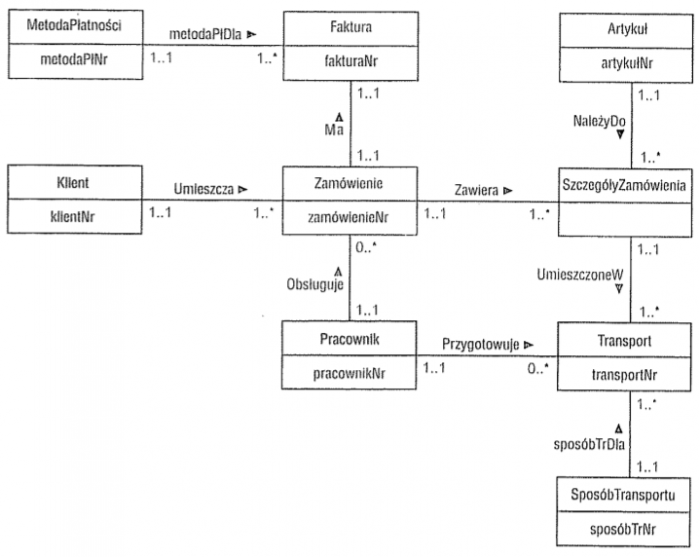
\includegraphics[scale=0.7]{7-4}

  \vspace{3cm}

  \begin{tabular}{|c|l|l|}
  \hline
  Nr & Encja & Relacje \\ \hline
  1 & Metoda płatności & \{\underline{metodaPłNr}\} \\ \hline
  2 & Faktura &\{\underline{fakturaNr}, metodaPłNr\} \\ \hline
  3 & Zamówienie & \{\underline{ZamówienieNr}, fakturaNr, metodaPłNr, klientNr, pracownikNr\} \\ \hline
  4 & Klient & \{\underline{klientNr}\} \\ \hline
  5 & Pracownik & \{\underline{pracownikNr}\} \\ \hline
  6 & Szczegóły zamówienia & \{\underline{zamówienieNr}, artykułNr\} \\ \hline
  7 & Transport & \{\underline{transportNr}, pracownikNr, zamówienieNr, sposóbNr\} \\ \hline
  8 & Sposób transportu & \{\underline{sposóbNr}\} \\ \hline
  9 & Artykuł & \{\underline{artykułNr}\} \\ \hline
  \end{tabular}
\end{center}

\newpage
\section{Zmodyfikuj poniższy model konceptualny usuwając z niego elementy niepożądane z punktu widzenia relacyjnego modelu danych. Wyznacz relacje dla poprawionego modelu.}
\begin{center}
	\includegraphics[scale=0.6]{mk-uml2}
\end{center}

\vspace{5mm}

\resizebox{175mm}{75mm}{%
% Graphic for TeX using PGF
% Title: /Users/evemorgen/Dropbox/studia/3rokEaiib/bazy_danych/lab7/7-5.dia
% Creator: Dia v0.97.2
% CreationDate: Tue Nov 22 23:38:44 2016
% For: evemorgen
% \usepackage{tikz}
% The following commands are not supported in PSTricks at present
% We define them conditionally, so when they are implemented,
% this pgf file will use them.
\ifx\du\undefined
  \newlength{\du}
\fi
\setlength{\du}{15\unitlength}
\begin{tikzpicture}
\pgftransformxscale{1.000000}
\pgftransformyscale{-1.000000}
\definecolor{dialinecolor}{rgb}{0.000000, 0.000000, 0.000000}
\pgfsetstrokecolor{dialinecolor}
\definecolor{dialinecolor}{rgb}{1.000000, 1.000000, 1.000000}
\pgfsetfillcolor{dialinecolor}
\pgfsetlinewidth{0.100000\du}
\pgfsetdash{}{0pt}
\definecolor{dialinecolor}{rgb}{1.000000, 1.000000, 1.000000}
\pgfsetfillcolor{dialinecolor}
\fill (20.730000\du,4.080000\du)--(20.730000\du,5.480000\du)--(25.465000\du,5.480000\du)--(25.465000\du,4.080000\du)--cycle;
\definecolor{dialinecolor}{rgb}{0.000000, 0.000000, 0.000000}
\pgfsetstrokecolor{dialinecolor}
\draw (20.730000\du,4.080000\du)--(20.730000\du,5.480000\du)--(25.465000\du,5.480000\du)--(25.465000\du,4.080000\du)--cycle;
% setfont left to latex
\definecolor{dialinecolor}{rgb}{0.000000, 0.000000, 0.000000}
\pgfsetstrokecolor{dialinecolor}
\node at (23.097500\du,5.080000\du){Personel};
\definecolor{dialinecolor}{rgb}{1.000000, 1.000000, 1.000000}
\pgfsetfillcolor{dialinecolor}
\fill (20.730000\du,5.480000\du)--(20.730000\du,6.480000\du)--(25.465000\du,6.480000\du)--(25.465000\du,5.480000\du)--cycle;
\definecolor{dialinecolor}{rgb}{0.000000, 0.000000, 0.000000}
\pgfsetstrokecolor{dialinecolor}
\draw (20.730000\du,5.480000\du)--(20.730000\du,6.480000\du)--(25.465000\du,6.480000\du)--(25.465000\du,5.480000\du)--cycle;
% setfont left to latex
\definecolor{dialinecolor}{rgb}{0.000000, 0.000000, 0.000000}
\pgfsetstrokecolor{dialinecolor}
\node[anchor=west] at (20.880000\du,6.180000\du){ personelNr};
\pgfsetlinewidth{0.100000\du}
\pgfsetdash{}{0pt}
\definecolor{dialinecolor}{rgb}{1.000000, 1.000000, 1.000000}
\pgfsetfillcolor{dialinecolor}
\fill (4.065000\du,9.940000\du)--(4.065000\du,11.340000\du)--(10.725000\du,11.340000\du)--(10.725000\du,9.940000\du)--cycle;
\definecolor{dialinecolor}{rgb}{0.000000, 0.000000, 0.000000}
\pgfsetstrokecolor{dialinecolor}
\draw (4.065000\du,9.940000\du)--(4.065000\du,11.340000\du)--(10.725000\du,11.340000\du)--(10.725000\du,9.940000\du)--cycle;
% setfont left to latex
\definecolor{dialinecolor}{rgb}{0.000000, 0.000000, 0.000000}
\pgfsetstrokecolor{dialinecolor}
\node at (7.395000\du,10.940000\du){Wlasciciel};
\definecolor{dialinecolor}{rgb}{1.000000, 1.000000, 1.000000}
\pgfsetfillcolor{dialinecolor}
\fill (4.065000\du,11.340000\du)--(4.065000\du,13.940000\du)--(10.725000\du,13.940000\du)--(10.725000\du,11.340000\du)--cycle;
\definecolor{dialinecolor}{rgb}{0.000000, 0.000000, 0.000000}
\pgfsetstrokecolor{dialinecolor}
\draw (4.065000\du,11.340000\du)--(4.065000\du,13.940000\du)--(10.725000\du,13.940000\du)--(10.725000\du,11.340000\du)--cycle;
% setfont left to latex
\definecolor{dialinecolor}{rgb}{0.000000, 0.000000, 0.000000}
\pgfsetstrokecolor{dialinecolor}
\node[anchor=west] at (4.215000\du,12.040000\du){ wlascicielNr};
% setfont left to latex
\definecolor{dialinecolor}{rgb}{0.000000, 0.000000, 0.000000}
\pgfsetstrokecolor{dialinecolor}
\node[anchor=west] at (4.215000\du,12.840000\du){ prywatny};
% setfont left to latex
\definecolor{dialinecolor}{rgb}{0.000000, 0.000000, 0.000000}
\pgfsetstrokecolor{dialinecolor}
\node[anchor=west] at (4.215000\du,13.640000\du){ instytucjonalny};
\pgfsetlinewidth{0.100000\du}
\pgfsetdash{}{0pt}
\definecolor{dialinecolor}{rgb}{1.000000, 1.000000, 1.000000}
\pgfsetfillcolor{dialinecolor}
\fill (19.665000\du,10.640000\du)--(19.665000\du,12.040000\du)--(26.547500\du,12.040000\du)--(26.547500\du,10.640000\du)--cycle;
\definecolor{dialinecolor}{rgb}{0.000000, 0.000000, 0.000000}
\pgfsetstrokecolor{dialinecolor}
\draw (19.665000\du,10.640000\du)--(19.665000\du,12.040000\du)--(26.547500\du,12.040000\du)--(26.547500\du,10.640000\du)--cycle;
% setfont left to latex
\definecolor{dialinecolor}{rgb}{0.000000, 0.000000, 0.000000}
\pgfsetstrokecolor{dialinecolor}
\node at (23.106250\du,11.640000\du){Nieruchomosc};
\definecolor{dialinecolor}{rgb}{1.000000, 1.000000, 1.000000}
\pgfsetfillcolor{dialinecolor}
\fill (19.665000\du,12.040000\du)--(19.665000\du,13.040000\du)--(26.547500\du,13.040000\du)--(26.547500\du,12.040000\du)--cycle;
\definecolor{dialinecolor}{rgb}{0.000000, 0.000000, 0.000000}
\pgfsetstrokecolor{dialinecolor}
\draw (19.665000\du,12.040000\du)--(19.665000\du,13.040000\du)--(26.547500\du,13.040000\du)--(26.547500\du,12.040000\du)--cycle;
% setfont left to latex
\definecolor{dialinecolor}{rgb}{0.000000, 0.000000, 0.000000}
\pgfsetstrokecolor{dialinecolor}
\node[anchor=west] at (19.815000\du,12.740000\du){ nieruchomoscNr};
\pgfsetlinewidth{0.100000\du}
\pgfsetdash{}{0pt}
\definecolor{dialinecolor}{rgb}{1.000000, 1.000000, 1.000000}
\pgfsetfillcolor{dialinecolor}
\fill (20.315000\du,17.390000\du)--(20.315000\du,18.790000\du)--(25.472500\du,18.790000\du)--(25.472500\du,17.390000\du)--cycle;
\definecolor{dialinecolor}{rgb}{0.000000, 0.000000, 0.000000}
\pgfsetstrokecolor{dialinecolor}
\draw (20.315000\du,17.390000\du)--(20.315000\du,18.790000\du)--(25.472500\du,18.790000\du)--(25.472500\du,17.390000\du)--cycle;
% setfont left to latex
\definecolor{dialinecolor}{rgb}{0.000000, 0.000000, 0.000000}
\pgfsetstrokecolor{dialinecolor}
\node at (22.893750\du,18.390000\du){Wynajecie};
\definecolor{dialinecolor}{rgb}{1.000000, 1.000000, 1.000000}
\pgfsetfillcolor{dialinecolor}
\fill (20.315000\du,18.790000\du)--(20.315000\du,19.790000\du)--(25.472500\du,19.790000\du)--(25.472500\du,18.790000\du)--cycle;
\definecolor{dialinecolor}{rgb}{0.000000, 0.000000, 0.000000}
\pgfsetstrokecolor{dialinecolor}
\draw (20.315000\du,18.790000\du)--(20.315000\du,19.790000\du)--(25.472500\du,19.790000\du)--(25.472500\du,18.790000\du)--cycle;
% setfont left to latex
\definecolor{dialinecolor}{rgb}{0.000000, 0.000000, 0.000000}
\pgfsetstrokecolor{dialinecolor}
\node[anchor=west] at (20.465000\du,19.490000\du){ wynajecieNr};
\pgfsetlinewidth{0.100000\du}
\pgfsetdash{}{0pt}
\definecolor{dialinecolor}{rgb}{1.000000, 1.000000, 1.000000}
\pgfsetfillcolor{dialinecolor}
\fill (34.865000\du,9.940000\du)--(34.865000\du,11.340000\du)--(39.600000\du,11.340000\du)--(39.600000\du,9.940000\du)--cycle;
\definecolor{dialinecolor}{rgb}{0.000000, 0.000000, 0.000000}
\pgfsetstrokecolor{dialinecolor}
\draw (34.865000\du,9.940000\du)--(34.865000\du,11.340000\du)--(39.600000\du,11.340000\du)--(39.600000\du,9.940000\du)--cycle;
% setfont left to latex
\definecolor{dialinecolor}{rgb}{0.000000, 0.000000, 0.000000}
\pgfsetstrokecolor{dialinecolor}
\node at (37.232500\du,10.940000\du){Wizyty};
\definecolor{dialinecolor}{rgb}{1.000000, 1.000000, 1.000000}
\pgfsetfillcolor{dialinecolor}
\fill (34.865000\du,11.340000\du)--(34.865000\du,13.140000\du)--(39.600000\du,13.140000\du)--(39.600000\du,11.340000\du)--cycle;
\definecolor{dialinecolor}{rgb}{0.000000, 0.000000, 0.000000}
\pgfsetstrokecolor{dialinecolor}
\draw (34.865000\du,11.340000\du)--(34.865000\du,13.140000\du)--(39.600000\du,13.140000\du)--(39.600000\du,11.340000\du)--cycle;
% setfont left to latex
\definecolor{dialinecolor}{rgb}{0.000000, 0.000000, 0.000000}
\pgfsetstrokecolor{dialinecolor}
\node[anchor=west] at (35.015000\du,12.040000\du){ dataWizyty};
% setfont left to latex
\definecolor{dialinecolor}{rgb}{0.000000, 0.000000, 0.000000}
\pgfsetstrokecolor{dialinecolor}
\node[anchor=west] at (35.015000\du,12.840000\du){ uwagi};
\pgfsetlinewidth{0.100000\du}
\pgfsetdash{}{0pt}
\definecolor{dialinecolor}{rgb}{1.000000, 1.000000, 1.000000}
\pgfsetfillcolor{dialinecolor}
\fill (34.765000\du,3.840000\du)--(34.765000\du,5.240000\du)--(39.885000\du,5.240000\du)--(39.885000\du,3.840000\du)--cycle;
\definecolor{dialinecolor}{rgb}{0.000000, 0.000000, 0.000000}
\pgfsetstrokecolor{dialinecolor}
\draw (34.765000\du,3.840000\du)--(34.765000\du,5.240000\du)--(39.885000\du,5.240000\du)--(39.885000\du,3.840000\du)--cycle;
% setfont left to latex
\definecolor{dialinecolor}{rgb}{0.000000, 0.000000, 0.000000}
\pgfsetstrokecolor{dialinecolor}
\node at (37.325000\du,4.840000\du){Klient};
\definecolor{dialinecolor}{rgb}{1.000000, 1.000000, 1.000000}
\pgfsetfillcolor{dialinecolor}
\fill (34.765000\du,5.240000\du)--(34.765000\du,7.040000\du)--(39.885000\du,7.040000\du)--(39.885000\du,5.240000\du)--cycle;
\definecolor{dialinecolor}{rgb}{0.000000, 0.000000, 0.000000}
\pgfsetstrokecolor{dialinecolor}
\draw (34.765000\du,5.240000\du)--(34.765000\du,7.040000\du)--(39.885000\du,7.040000\du)--(39.885000\du,5.240000\du)--cycle;
% setfont left to latex
\definecolor{dialinecolor}{rgb}{0.000000, 0.000000, 0.000000}
\pgfsetstrokecolor{dialinecolor}
\node[anchor=west] at (34.915000\du,5.940000\du){ kleintNr};
% setfont left to latex
\definecolor{dialinecolor}{rgb}{0.000000, 0.000000, 0.000000}
\pgfsetstrokecolor{dialinecolor}
\node[anchor=west] at (34.915000\du,6.740000\du){ preferencje};
\pgfsetlinewidth{0.100000\du}
\pgfsetdash{}{0pt}
\pgfsetmiterjoin
\pgfsetbuttcap
{
\definecolor{dialinecolor}{rgb}{0.000000, 0.000000, 0.000000}
\pgfsetfillcolor{dialinecolor}
% was here!!!
\definecolor{dialinecolor}{rgb}{0.000000, 0.000000, 0.000000}
\pgfsetstrokecolor{dialinecolor}
\draw (10.725000\du,11.840000\du)--(10.775000\du,11.840000\du)--(19.564574\du,11.840000\du)--(19.614574\du,11.840000\du);
}
% setfont left to latex
\definecolor{dialinecolor}{rgb}{0.000000, 0.000000, 0.000000}
\pgfsetstrokecolor{dialinecolor}
\node at (15.169787\du,11.690000\du){posiada};
\definecolor{dialinecolor}{rgb}{0.000000, 0.000000, 0.000000}
\pgfsetfillcolor{dialinecolor}
\fill (16.617287\du,11.690000\du)--(16.617287\du,11.290000\du)--(17.017287\du,11.490000\du)--cycle;
% setfont left to latex
\definecolor{dialinecolor}{rgb}{0.000000, 0.000000, 0.000000}
\pgfsetstrokecolor{dialinecolor}
\node[anchor=west] at (11.000000\du,11.600000\du){0..1};
% setfont left to latex
\definecolor{dialinecolor}{rgb}{0.000000, 0.000000, 0.000000}
\pgfsetstrokecolor{dialinecolor}
\node[anchor=west] at (18.100000\du,11.650000\du){1..*};
\pgfsetlinewidth{0.100000\du}
\pgfsetdash{}{0pt}
\pgfsetmiterjoin
\pgfsetbuttcap
{
\definecolor{dialinecolor}{rgb}{0.000000, 0.000000, 0.000000}
\pgfsetfillcolor{dialinecolor}
% was here!!!
\definecolor{dialinecolor}{rgb}{0.000000, 0.000000, 0.000000}
\pgfsetstrokecolor{dialinecolor}
\draw (23.097500\du,6.480000\du)--(23.097500\du,8.800000\du)--(23.106250\du,8.800000\du)--(23.106250\du,10.589785\du);
}
% setfont left to latex
\definecolor{dialinecolor}{rgb}{0.000000, 0.000000, 0.000000}
\pgfsetstrokecolor{dialinecolor}
\node at (23.101875\du,8.650000\du){         zarzadza};
\definecolor{dialinecolor}{rgb}{0.000000, 0.000000, 0.000000}
\pgfsetfillcolor{dialinecolor}
\fill (26.474375\du,8.650000\du)--(26.474375\du,8.250000\du)--(26.874375\du,8.450000\du)--cycle;
% setfont left to latex
\definecolor{dialinecolor}{rgb}{0.000000, 0.000000, 0.000000}
\pgfsetstrokecolor{dialinecolor}
\node[anchor=west] at (23.300000\du,7.200000\du){0..1};
% setfont left to latex
\definecolor{dialinecolor}{rgb}{0.000000, 0.000000, 0.000000}
\pgfsetstrokecolor{dialinecolor}
\node[anchor=west] at (23.350000\du,10.350000\du){0..100};
\pgfsetlinewidth{0.100000\du}
\pgfsetdash{}{0pt}
\pgfsetmiterjoin
\pgfsetbuttcap
{
\definecolor{dialinecolor}{rgb}{0.000000, 0.000000, 0.000000}
\pgfsetfillcolor{dialinecolor}
% was here!!!
\definecolor{dialinecolor}{rgb}{0.000000, 0.000000, 0.000000}
\pgfsetstrokecolor{dialinecolor}
\draw (34.865000\du,11.840000\du)--(34.815000\du,11.840000\du)--(26.647926\du,11.840000\du)--(26.597926\du,11.840000\du);
}
% setfont left to latex
\definecolor{dialinecolor}{rgb}{0.000000, 0.000000, 0.000000}
\pgfsetstrokecolor{dialinecolor}
\node at (30.731463\du,11.690000\du){odbywa się};
\definecolor{dialinecolor}{rgb}{0.000000, 0.000000, 0.000000}
\pgfsetfillcolor{dialinecolor}
\fill (32.756463\du,11.690000\du)--(32.756463\du,11.290000\du)--(33.156463\du,11.490000\du)--cycle;
\pgfsetlinewidth{0.100000\du}
\pgfsetdash{}{0pt}
\pgfsetmiterjoin
\pgfsetbuttcap
{
\definecolor{dialinecolor}{rgb}{0.000000, 0.000000, 0.000000}
\pgfsetfillcolor{dialinecolor}
% was here!!!
\definecolor{dialinecolor}{rgb}{0.000000, 0.000000, 0.000000}
\pgfsetstrokecolor{dialinecolor}
\draw (39.600000\du,11.840000\du)--(41.900000\du,11.840000\du)--(41.900000\du,5.440000\du)--(39.934738\du,5.440000\du);
}
% setfont left to latex
\definecolor{dialinecolor}{rgb}{0.000000, 0.000000, 0.000000}
\pgfsetstrokecolor{dialinecolor}
\node[anchor=west] at (42.000000\du,8.490000\du){zamawia};
\definecolor{dialinecolor}{rgb}{0.000000, 0.000000, 0.000000}
\pgfsetfillcolor{dialinecolor}
\fill (44.795000\du,8.490000\du)--(44.795000\du,8.090000\du)--(45.195000\du,8.290000\du)--cycle;
\pgfsetlinewidth{0.100000\du}
\pgfsetdash{}{0pt}
\pgfsetmiterjoin
\pgfsetbuttcap
{
\definecolor{dialinecolor}{rgb}{0.000000, 0.000000, 0.000000}
\pgfsetfillcolor{dialinecolor}
% was here!!!
\definecolor{dialinecolor}{rgb}{0.000000, 0.000000, 0.000000}
\pgfsetstrokecolor{dialinecolor}
\draw (25.650000\du,5.450000\du)--(28.150000\du,5.450000\du)--(28.150000\du,5.440000\du)--(34.714851\du,5.440000\du);
}
% setfont left to latex
\definecolor{dialinecolor}{rgb}{0.000000, 0.000000, 0.000000}
\pgfsetstrokecolor{dialinecolor}
\node[anchor=west] at (28.250000\du,5.295000\du){rejestruje};
\definecolor{dialinecolor}{rgb}{0.000000, 0.000000, 0.000000}
\pgfsetfillcolor{dialinecolor}
\fill (32.200000\du,5.295000\du)--(32.200000\du,4.895000\du)--(32.600000\du,5.095000\du)--cycle;
\pgfsetlinewidth{0.100000\du}
\pgfsetdash{}{0pt}
\pgfsetmiterjoin
\pgfsetbuttcap
{
\definecolor{dialinecolor}{rgb}{0.000000, 0.000000, 0.000000}
\pgfsetfillcolor{dialinecolor}
% was here!!!
\definecolor{dialinecolor}{rgb}{0.000000, 0.000000, 0.000000}
\pgfsetstrokecolor{dialinecolor}
\draw (22.900000\du,13.150000\du)--(22.900000\du,15.244847\du)--(22.893750\du,15.244847\du)--(22.893750\du,17.339695\du);
}
% setfont left to latex
\definecolor{dialinecolor}{rgb}{0.000000, 0.000000, 0.000000}
\pgfsetstrokecolor{dialinecolor}
\node at (22.896875\du,15.094847\du){jest skojarzona z};
\definecolor{dialinecolor}{rgb}{0.000000, 0.000000, 0.000000}
\pgfsetfillcolor{dialinecolor}
\fill (26.269375\du,15.094847\du)--(26.269375\du,14.694847\du)--(26.669375\du,14.894847\du)--cycle;
\pgfsetlinewidth{0.100000\du}
\pgfsetdash{}{0pt}
\pgfsetmiterjoin
\pgfsetbuttcap
{
\definecolor{dialinecolor}{rgb}{0.000000, 0.000000, 0.000000}
\pgfsetfillcolor{dialinecolor}
% was here!!!
\definecolor{dialinecolor}{rgb}{0.000000, 0.000000, 0.000000}
\pgfsetstrokecolor{dialinecolor}
\draw (39.885000\du,4.540000\du)--(45.450000\du,4.540000\du)--(45.450000\du,18.590000\du)--(25.521917\du,18.590000\du);
}
% setfont left to latex
\definecolor{dialinecolor}{rgb}{0.000000, 0.000000, 0.000000}
\pgfsetstrokecolor{dialinecolor}
\node[anchor=west] at (45.550000\du,11.415000\du){wynajmuje};
\definecolor{dialinecolor}{rgb}{0.000000, 0.000000, 0.000000}
\pgfsetfillcolor{dialinecolor}
\fill (49.115000\du,11.415000\du)--(49.115000\du,11.015000\du)--(49.515000\du,11.215000\du)--cycle;
\pgfsetlinewidth{0.100000\du}
\pgfsetdash{}{0pt}
\definecolor{dialinecolor}{rgb}{1.000000, 1.000000, 1.000000}
\pgfsetfillcolor{dialinecolor}
\fill (20.465000\du,-3.610000\du)--(20.465000\du,-2.210000\du)--(25.947500\du,-2.210000\du)--(25.947500\du,-3.610000\du)--cycle;
\definecolor{dialinecolor}{rgb}{0.000000, 0.000000, 0.000000}
\pgfsetstrokecolor{dialinecolor}
\draw (20.465000\du,-3.610000\du)--(20.465000\du,-2.210000\du)--(25.947500\du,-2.210000\du)--(25.947500\du,-3.610000\du)--cycle;
% setfont left to latex
\definecolor{dialinecolor}{rgb}{0.000000, 0.000000, 0.000000}
\pgfsetstrokecolor{dialinecolor}
\node at (23.206250\du,-2.610000\du){kierowanie};
\definecolor{dialinecolor}{rgb}{1.000000, 1.000000, 1.000000}
\pgfsetfillcolor{dialinecolor}
\fill (20.465000\du,-2.210000\du)--(20.465000\du,-1.810000\du)--(25.947500\du,-1.810000\du)--(25.947500\du,-2.210000\du)--cycle;
\definecolor{dialinecolor}{rgb}{0.000000, 0.000000, 0.000000}
\pgfsetstrokecolor{dialinecolor}
\draw (20.465000\du,-2.210000\du)--(20.465000\du,-1.810000\du)--(25.947500\du,-1.810000\du)--(25.947500\du,-2.210000\du)--cycle;
\pgfsetlinewidth{0.100000\du}
\pgfsetdash{}{0pt}
\pgfsetmiterjoin
\pgfsetbuttcap
{
\definecolor{dialinecolor}{rgb}{0.000000, 0.000000, 0.000000}
\pgfsetfillcolor{dialinecolor}
% was here!!!
\definecolor{dialinecolor}{rgb}{0.000000, 0.000000, 0.000000}
\pgfsetstrokecolor{dialinecolor}
\draw (25.200000\du,-1.750000\du)--(25.200000\du,-1.700000\du)--(25.200000\du,3.950000\du)--(25.200000\du,4.000000\du);
}
% setfont left to latex
\definecolor{dialinecolor}{rgb}{0.000000, 0.000000, 0.000000}
\pgfsetstrokecolor{dialinecolor}
\node[anchor=west] at (25.300000\du,0.975000\du){kierowanyPrzez};
\definecolor{dialinecolor}{rgb}{0.000000, 0.000000, 0.000000}
\pgfsetfillcolor{dialinecolor}
\fill (30.790000\du,0.975000\du)--(30.790000\du,0.575000\du)--(31.190000\du,0.775000\du)--cycle;
\pgfsetlinewidth{0.100000\du}
\pgfsetdash{}{0pt}
\pgfsetmiterjoin
\pgfsetbuttcap
{
\definecolor{dialinecolor}{rgb}{0.000000, 0.000000, 0.000000}
\pgfsetfillcolor{dialinecolor}
% was here!!!
\definecolor{dialinecolor}{rgb}{0.000000, 0.000000, 0.000000}
\pgfsetstrokecolor{dialinecolor}
\draw (21.115000\du,-1.760000\du)--(21.115000\du,-1.710000\du)--(21.115000\du,3.940000\du)--(21.115000\du,3.990000\du);
}
% setfont left to latex
\definecolor{dialinecolor}{rgb}{0.000000, 0.000000, 0.000000}
\pgfsetstrokecolor{dialinecolor}
\node[anchor=west] at (21.215000\du,0.965000\du){kieruje};
\definecolor{dialinecolor}{rgb}{0.000000, 0.000000, 0.000000}
\pgfsetfillcolor{dialinecolor}
\fill (24.010000\du,0.965000\du)--(24.010000\du,0.565000\du)--(24.410000\du,0.765000\du)--cycle;
% setfont left to latex
\definecolor{dialinecolor}{rgb}{0.000000, 0.000000, 0.000000}
\pgfsetstrokecolor{dialinecolor}
\node[anchor=west] at (21.200000\du,-1.100000\du){0..*};
% setfont left to latex
\definecolor{dialinecolor}{rgb}{0.000000, 0.000000, 0.000000}
\pgfsetstrokecolor{dialinecolor}
\node[anchor=west] at (23.700000\du,-1.050000\du){0..*};
% setfont left to latex
\definecolor{dialinecolor}{rgb}{0.000000, 0.000000, 0.000000}
\pgfsetstrokecolor{dialinecolor}
\node[anchor=west] at (21.300000\du,3.850000\du){1..1};
% setfont left to latex
\definecolor{dialinecolor}{rgb}{0.000000, 0.000000, 0.000000}
\pgfsetstrokecolor{dialinecolor}
\node[anchor=west] at (23.800000\du,3.800000\du){1..1};
% setfont left to latex
\definecolor{dialinecolor}{rgb}{0.000000, 0.000000, 0.000000}
\pgfsetstrokecolor{dialinecolor}
\node[anchor=west] at (23.200000\du,13.750000\du){1..1};
% setfont left to latex
\definecolor{dialinecolor}{rgb}{0.000000, 0.000000, 0.000000}
\pgfsetstrokecolor{dialinecolor}
\node[anchor=west] at (23.150000\du,17.000000\du){0..*};
% setfont left to latex
\definecolor{dialinecolor}{rgb}{0.000000, 0.000000, 0.000000}
\pgfsetstrokecolor{dialinecolor}
\node[anchor=west] at (25.650000\du,18.350000\du){0..*};
% setfont left to latex
\definecolor{dialinecolor}{rgb}{0.000000, 0.000000, 0.000000}
\pgfsetstrokecolor{dialinecolor}
\node[anchor=west] at (40.300000\du,4.300000\du){1..1};
% setfont left to latex
\definecolor{dialinecolor}{rgb}{0.000000, 0.000000, 0.000000}
\pgfsetstrokecolor{dialinecolor}
\node[anchor=west] at (33.500000\du,11.600000\du){1..1};
% setfont left to latex
\definecolor{dialinecolor}{rgb}{0.000000, 0.000000, 0.000000}
\pgfsetstrokecolor{dialinecolor}
\node[anchor=west] at (39.750000\du,11.500000\du){1..1};
% setfont left to latex
\definecolor{dialinecolor}{rgb}{0.000000, 0.000000, 0.000000}
\pgfsetstrokecolor{dialinecolor}
\node[anchor=west] at (40.100000\du,6.300000\du){0..*};
% setfont left to latex
\definecolor{dialinecolor}{rgb}{0.000000, 0.000000, 0.000000}
\pgfsetstrokecolor{dialinecolor}
\node[anchor=west] at (33.350000\du,5.300000\du){0..*};
% setfont left to latex
\definecolor{dialinecolor}{rgb}{0.000000, 0.000000, 0.000000}
\pgfsetstrokecolor{dialinecolor}
\node[anchor=west] at (25.600000\du,5.250000\du){1..1};
\end{tikzpicture}

}

\vspace{5mm}

\begin{center}
  \begin{tabular}{|c|l|l|}
    \hline
    Nr & Encja & Relacje \\ \hline
    1 & Właściciel & \{\underline{właścicielNr}\} \\ \hline
    2 & Nieruchomość &\{\underline{nieruchomośćNr}, właścicielNr, personelNr\} \\ \hline
    3 & Personel & \{\underline{personelNr}, kientNr\} \\ \hline
    4 & Kierowanie & \{\} \\ \hline
    5 & Klient & \{\underline{kientNr}, preferencje\} \\ \hline
    6 & Wizyty & \{data wizyty, uwagi, nieruchomośćNr, kientNr\} \\ \hline
    7 & Wynajęcie & \{\underline{wynajęcieNr}, nieruchomośćNr, kientNr\} \\ \hline
  \end{tabular}
\end{center}

\end{document}
